\section{Algorithm}
%
The most straightforward approach to extracting the surface from a binary image mask is simply applying the marching cubes algorithm. As alluded to in the introduction, though, surfaces generated by marching cubes alone are inadequate for simulation purposes. Specifically, surfaces of this kind exhibit a ``Lego-like'' appearance that is visually displeasing, poorly represents the original object being scanned, and makes the resulting surface unacceptable for any simulation involving contact. Thus, the surface must be smoothed - ideally using a technique that attempts to preserve the volume of the original object such as \textit{HC Laplacian smoothing}~\cite{vollmer_1999} or \textit{Taubin smoothing}~\cite{taubin_1995}. Nonetheless, the step-like appearance of surfaces extracted by marching cubes often requires a degree of smoothing that causes a significant loss in features and/or the surface to become non-manifold. Sophisticated surface generation techniques attempt to generate a surface that preserves both the smooth and sharp features of the original object. \\ \\
Labsik \textit{et al.}~\cite{labsik_2002} extracted a coarse resolution surface using marching cubes, followed by iteratively remeshing to finer resolutions where features exist. Kobbelt \textit{et al.}~\cite{kobbelt_2001} retained sharp features from binary image masks by modifying the marching cubes algorithm in two ways: by enhancing the discrete distance field that defines the underlying isosurface of the image mask, and by adding additional sample points to detect edges and corners. Depending on the application, though, surface smoothness may well be more important than sharp feature preservation. Lempitsky~\cite{lempitsky_2010}, for example, enforced higher-order smoothness by modifying the isosurface function and solving a convex quadratic optimization problem for each grid cell. \\ \\ 
The novel approach outlined herein involves generating a high-quality point cloud that approximates the boundary, followed by a surface reconstruction technique based on Voronoi partitioning. \textit{Surface reconstruction} is the process of generating watertight, explicit, manifold surfaces from \textit{point cloud} data. The approach attempts to create smooth surfaces without over-smoothing, and it can be extended to capture sharp features as well.
%%%%%%%%%%%%%%%%%%%%%%%%%%%%%%%%%%%%%%%%%%%%%%%
%%%%%%%%%%%%%%%%%%%%%%%%%%%%%%%%%%%%%%%%%%%%%%%
\subsection{Point Cloud Generation}
\label{Point Cloud Generation}

A \textit{segmented image} or \textit{image mask} is a 3D structured array of voxels, each of which has been assigned an identifier
that indicates a material type (or in the case of no material, void). We confine attention to the single-material case, and take the segmented image as our starting point.  Given a segmented image, we seek to generate a {\em boundary representation} (b-rep) for the region occupied by material, i.e., the solid body.  This b-rep takes the form of a connected, watertight collection of polygonal facets.  In our approach, Voronoi tessellation is central to the creation of the b-rep, for which an {\em oriented point cloud} is required.  We therefore first focus on the generation of an oriented point cloud on the surface of the material body, given a segmented image. \\ \\
%
A point cloud is oriented if the surface normal data is included at each point, in addition to the point's spatial coordinates. To compute the point cloud, the image mask is sampled with small, overlapping \textit{windows} to locally approximate the material boundary. For each three-dimensional window, the following tasks are performed:
\vspace{3mm}
\begin{itemize}[noitemsep]
  \item Determine whether the window intersects the material boundary.
  \item Locally approximate the boundary via an optimization problem. 
  \item Place a point and associated normal on the approximated boundary surface.
\end{itemize}
\vspace{3mm}
The basic sequence is shown (in 2D for clarity) in panels (a-c) of~\figref{vor}. Each step in the generation of the oriented point cloud is described in the subsections below.

\begin{figure}[ht]
\centering
\subfigure[]{%
		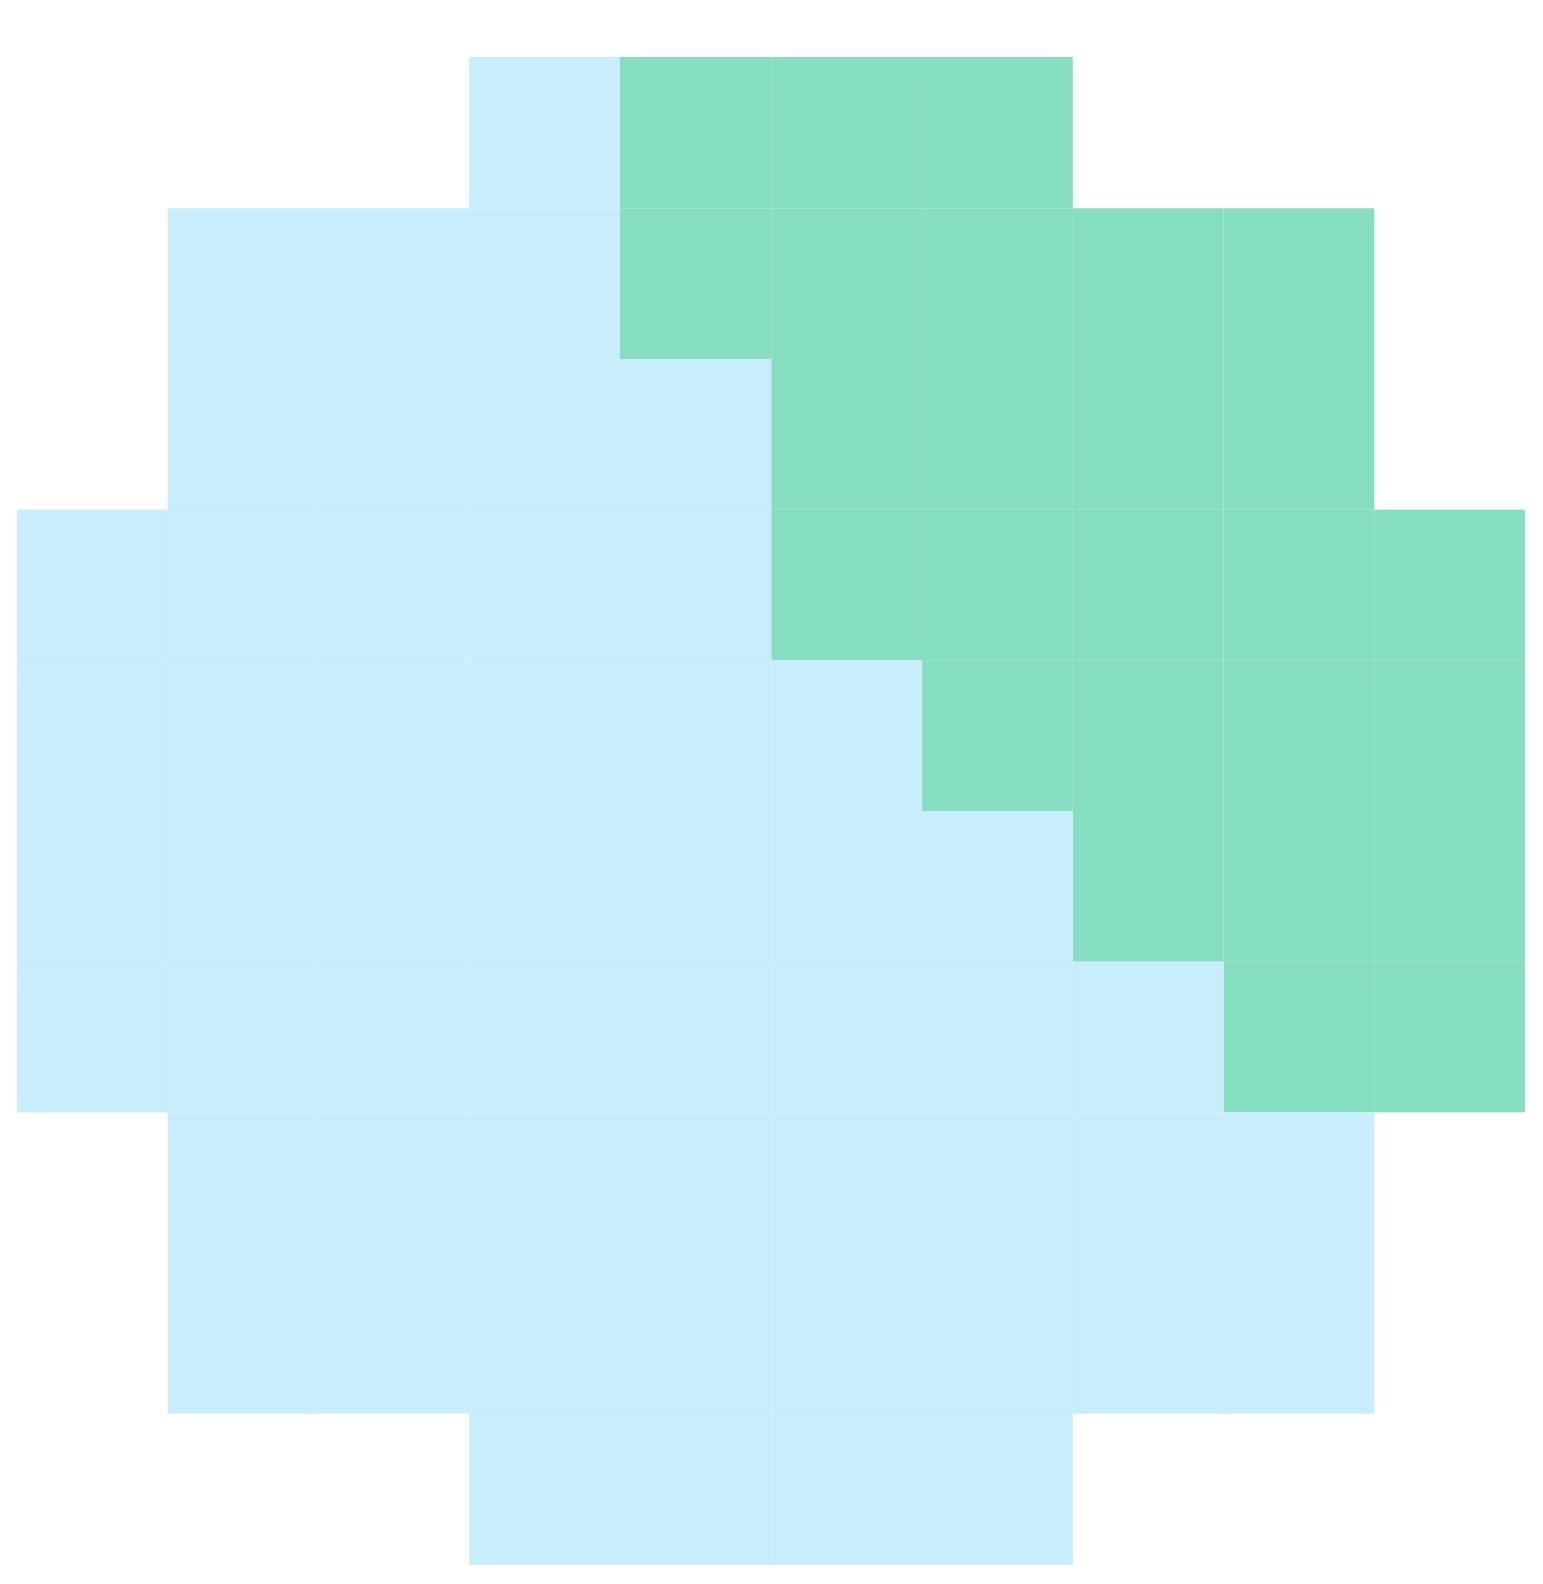
\includegraphics[scale=0.57]{media/2-shabaka/1-vor/dem1.png}
\label{fig:vor1}}
\subfigure[]{%
		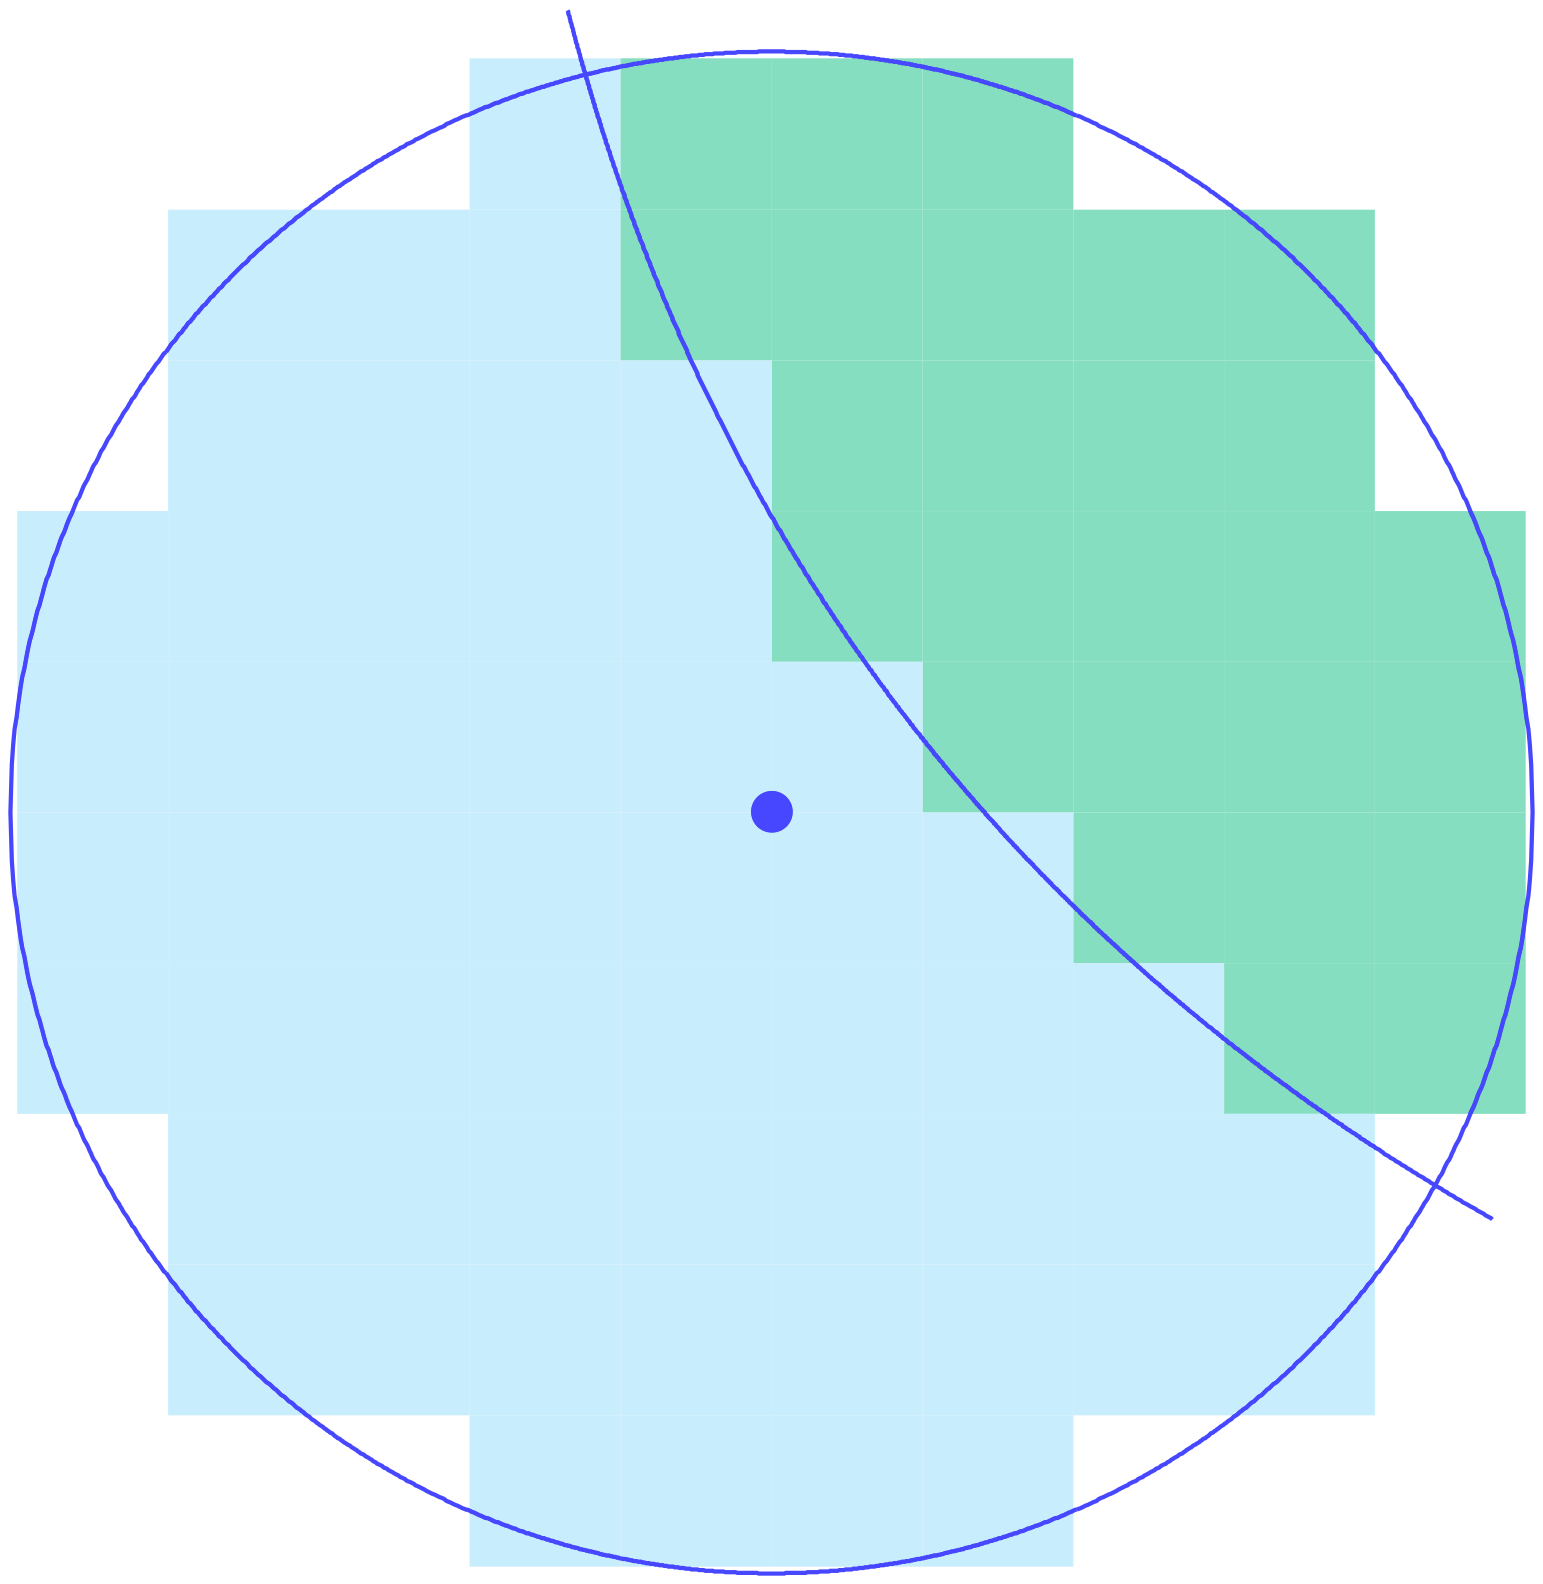
\includegraphics[scale=0.57]{media/2-shabaka/1-vor/dem2.png}
\label{fig:vor2}}
\subfigure[]{%
		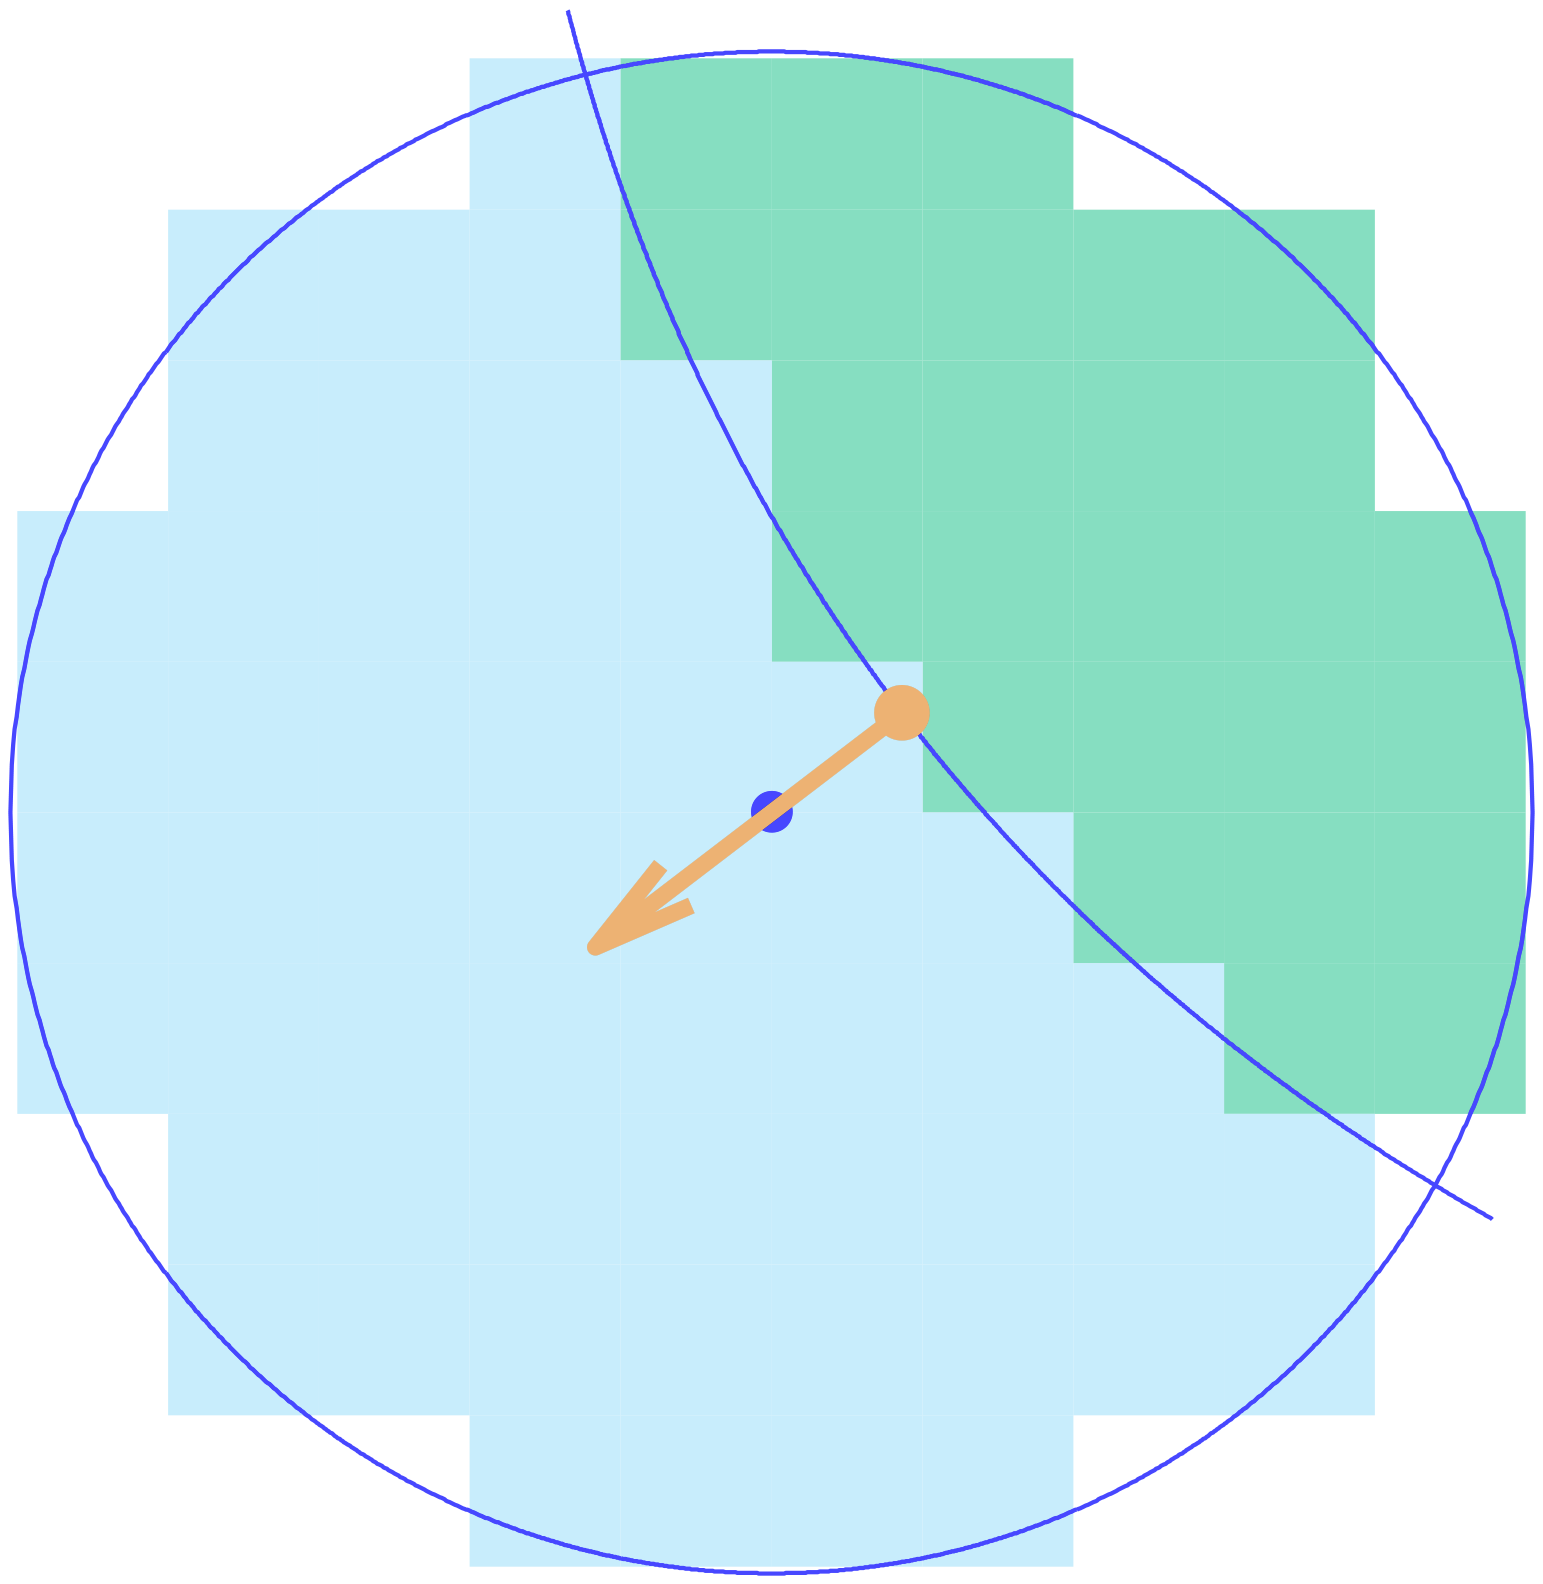
\includegraphics[scale=0.57]{media/2-shabaka/1-vor/dem3.png}
\label{fig:vor3}}
\subfigure[]{%
		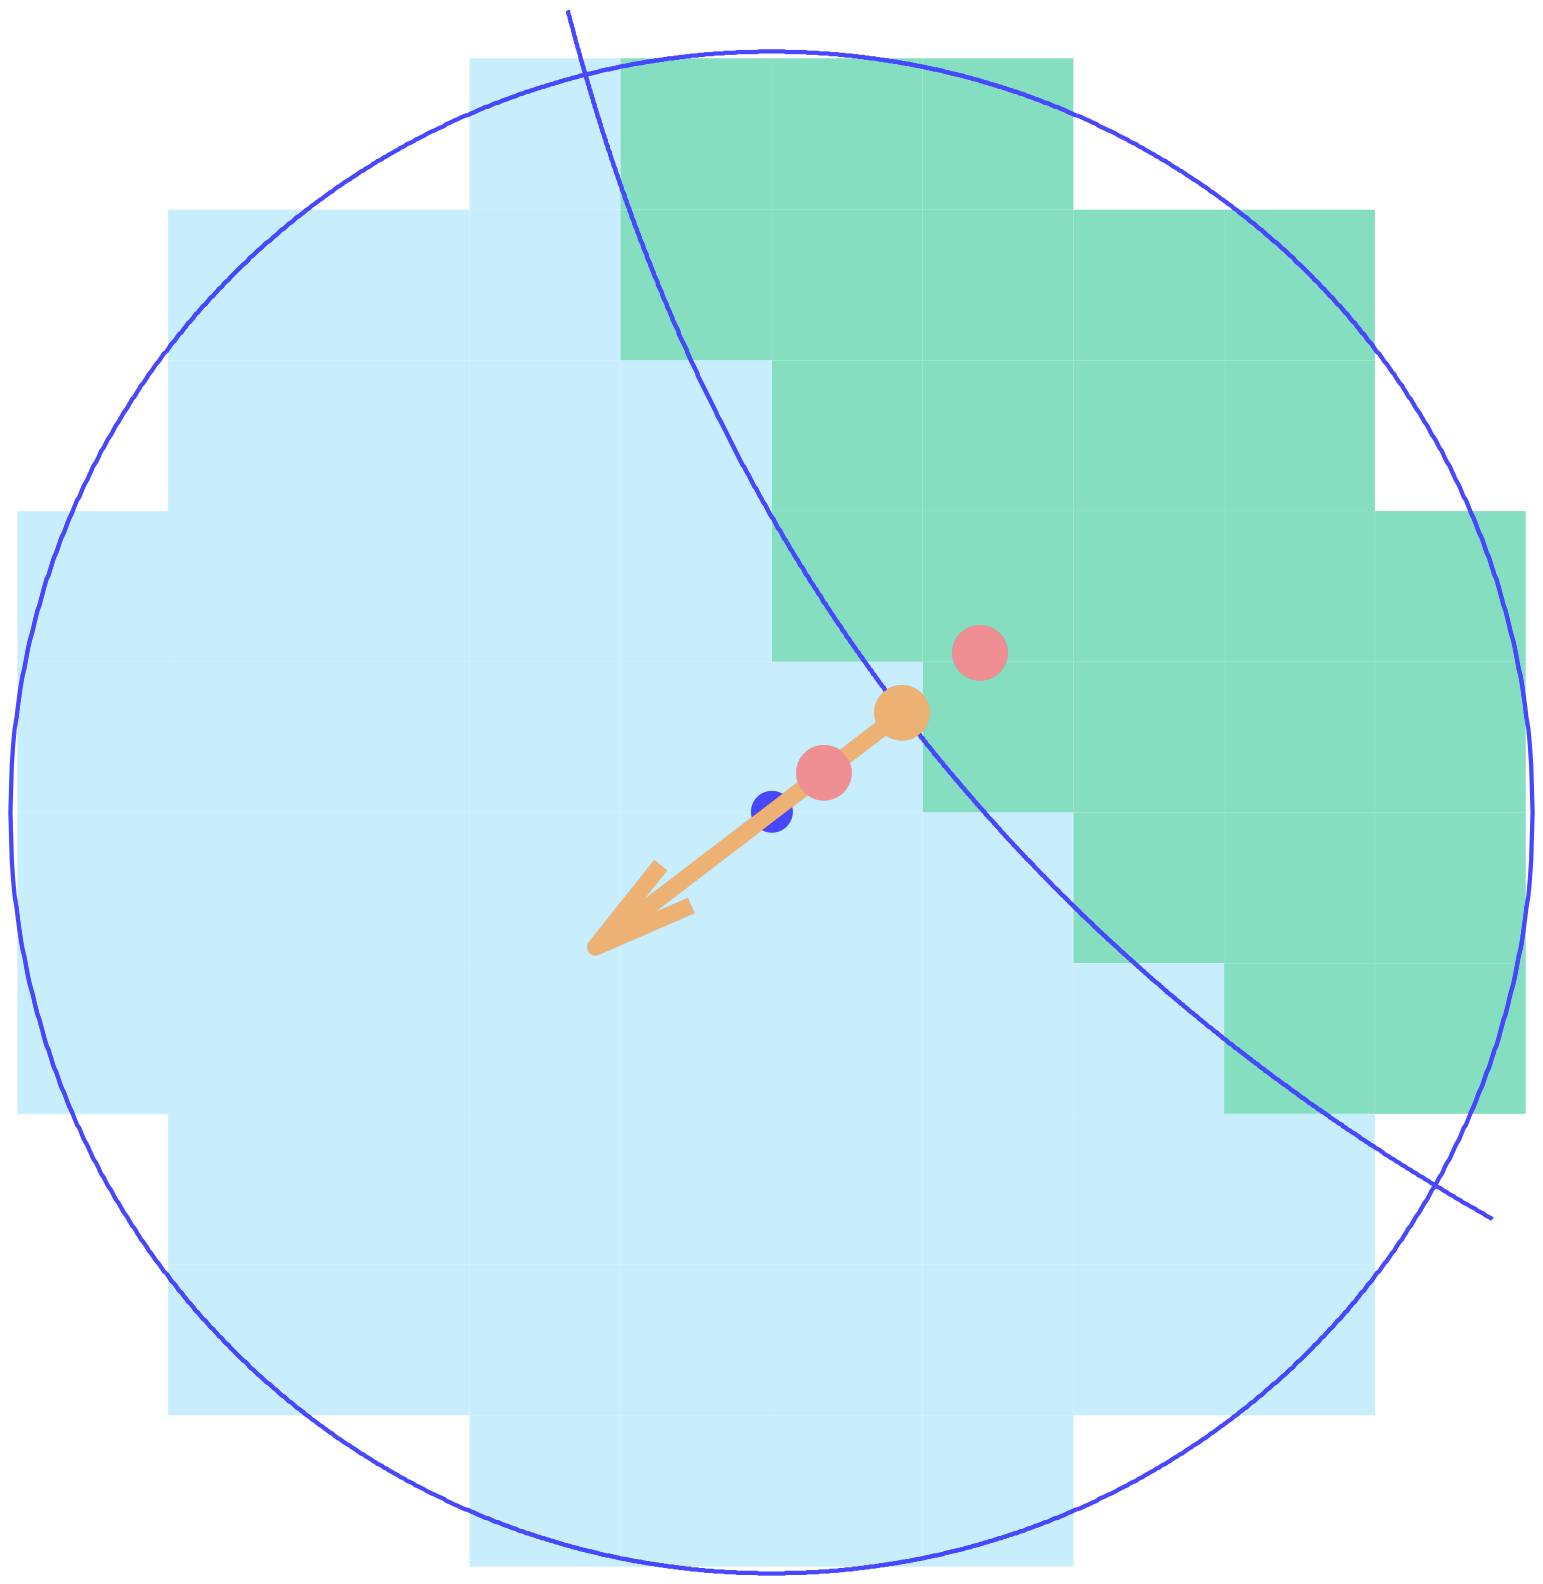
\includegraphics[scale=0.57]{media/2-shabaka/1-vor/dem4.png}
\label{fig:vor4}}
%
\caption{(a) Sampling window of segmented image, (b) boundary approximation, (c) point/normal placement, and d) Voronoi site placement. Green voxels indicate solid material and blue voxels are void.}
\label{fig:vor}
\end{figure}

\subsubsection{Window Selection}

We denote the set of all voxels in a segmented image as $\mathcal{I}$. The segmented image  $\mathcal{I}$ is sampled with overlapping windows, each of which is a voxelized sphere with voxel radius $R_{\mathcal{W}}$ (an integer). The translation in each Cartesian direction between adjacent windows is $d_{\mathcal{W}}$, which is also an integer voxel count. The set of voxels in a particular window is defined as $\mathcal{W}$, and the number of voxels in that window is $n_{\mathcal{W}}$. We further define the subset of voxels in $\mathcal{W}$ that are designated as solid material to be $\mathcal{M}$, with $n_{\mc{M}} = | \mc{M} |$. \\ \\
%
A window $\mathcal{W}$ is marked for further processing if it satisfies a threshold requirement, as follows.  Letting $k_{\mathcal{M}} = n_{\mathcal{M}}/n_{\mathcal{W}}$, we define a threshold value $\overline{k}_{\mathcal{M}}$ such that the window is retained only if $k_{\mathcal{M}} \in (\overline{k}_{\mathcal{M}}, 1 - \overline{k}_{\mc{M}})$.  Thus, further calculations are performed only if sufficiently many voxels of both solid material and of void are present in the window to support approximation of a material boundary. Refer to~\tabref{window} for a summary of these variables and their descriptions. 

\begin{table}[htbp!]
 \centering
   \begin{tabular}{|c||c|}
   \hline
   {\textbf{Variable}} & \textbf{Description} \\ \hline \hline
   $\mathcal{I}$ & set of all voxels in a segmented image \\ \hline
   $\mathcal{W}$ & set of all voxels in a window \\ \hline
   $\mc{M}$ & subset of $\mc{W}$ occupied by material \\ \hline
   {$k_{\mathcal{M}}$} & ratio of voxels in $\mathcal{M}$ to voxels in $\mathcal{W}$\\ \hline
   {$\overline{k}_{\mathcal{M}}$ \rule{0mm}{4mm}} & threshold value for $k_{\mathcal{M}}$ \\ \hline 
   $R_{\mathcal{W}}$ & window radius (in voxels) \\ \hline
   $d_{\mathcal{W}}$ & sampling distance between adjacent windows (in voxels) \\ \hline  
\end{tabular}
\caption{List of variables for window selection}
\label{tab:window}
\end{table}

\subsubsection{Local Boundary Approximation}

Given a window $\mathcal{W}$ that is marked as intersecting the body boundary, we seek to derive a local boundary-surface patch $\mc{S}$ that optimally represents the boundary separating $\mc{M}$ and $\mc{W} \setminus \mc{M}$.  The overall plan is as follows: we define geometrically smooth (i.e., not voxelated), disjoint, simply-connected regions that approximate $\mc{W}$ and $\mc{M}$, whose common boundary serves to define the surface patch $\mc{S}$.  The regions and the surface $\mc{S}$ are taken to have simple, parameterizable shapes; optimally fitting them to $\mc{W}$ and $\mc{M}$ therefore reduces to a small algebraic minimization problem.  We require that $\mc{S}$ be non-intersecting, and that it divides the smooth approximation to $\mc{W}$ into exactly two subregions. \\ \\
%
Proceeding in this direction, let $\mc{D}$ be a sphere whose center and radius $R$ are chosen so that the centroid and volume of $D$ match those of $\mc{W}$.  Next, we define $\Omega_p$ as the spatial region occupied by $\mc{M}$, and $\Omega$ as the subset of $\mc{D}$ that lies on one side of $\mc{S}$.  We assume that $\mc{S}$ intersects $\partial \mc{D}$ in a simple closed loop, so that $\Omega$ is a simply-connected subset of $\mc{D}$ that resembles a ``lens.''  The situation is illustrated in~\figref{figure3}. \\ \\
%
It remains to provide a concrete parameterization of $\mc{S}$, and a specific objective function through which $\Omega$ is optimally fitted to $\Omega_p$.  To these ends, in this initial exposition we take $\mc{S}$ to be planar, as shown in \figref{quad}, and we define an objective function via the zeroth, first, and second moments of volume of $\Omega$ and $\Omega_p$: 
\begin{alignat}{5}
&{} &&V^p = \int_{\Omega_p}dv, &&{} \\
I_{x\phantom{z}}^p &= \int_{\Omega_p}xdv, &&I_{y\phantom{z}}^p = \int_{\Omega_p}ydv, &&I_{z\phantom{z}}^p = \int_{\Omega_p}zdv, \\
I^p_{xy} &= \int_{\Omega_p}xydv, &&I^p_{xz} = \int_{\Omega_p}xzdv, &&I^p_{yz} = \int_{\Omega_p}yzdv, \\
I^p_{xx} &= \int_{\Omega_p}(y^2 + z^2)dv, \text{\ \ \ \ \ \ }&&I^p_{yy} = \int_{\Omega_p}(x^2 + z^2)dv, \text{\ \ \ \ \ \ }&&I^p_{zz} = \int_{\Omega_p}(x^2 + y^2)dv.
\end{alignat}
Analogous quantities $V$, $I_x$, etc. are defined for $\Omega$.  Taking the coordinate origin to be the common centroid of $\Omega$ and $\Omega_p$, the planar surface $\mc{S}$ is defined by $x' = d$, where the primed coordinates are oriented such that the $x'$ axis is normal to $\mc{S}$, as shown in \figref{quad}.  In three dimensions, the transformation matrix between primed and unprimed Cartesian frames is given in terms of the polar angles $\psi, \theta$ by:
\begin{gather}
\bm{R} = \left[\begin{array} {ccc} {\cos\psi\cos\theta} & {-\sin\psi} & {\cos\psi\sin\theta}\\ {\sin\psi\cos\theta} & {\cos\psi} & {\sin\psi\sin\theta}, \\
{-\sin\theta} & {0} & {\cos\theta}\end{array} \right].
\end{gather}


\begin{figure}[ht]
\centering
\subfigure[Window $\mathcal{W}$]{%
		
\includegraphics[scale=0.72]{media/om/dem2.pdf}
\label{fig:subfigure2}}
\subfigure[Approximating sphere $\mathcal{D}$]{%
		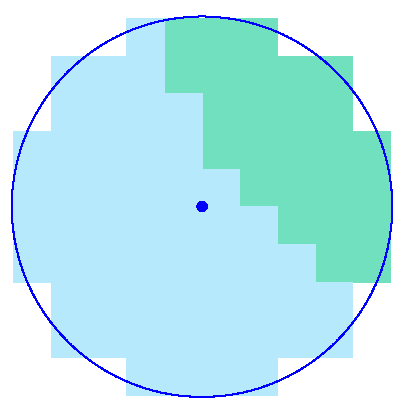
\includegraphics[scale=0.72]{media/om/dem3.pdf}
\label{fig:subfigure3}}

\subfigure[Approximating surface $\mathcal{S}$]{%
		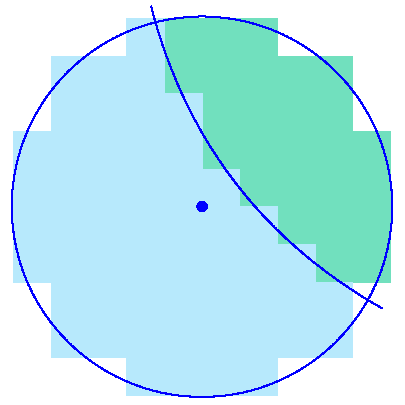
\includegraphics[scale=0.72]{media/om/dem4.pdf}
\label{fig:subfigure4}}
\subfigure[Voxelated region $\Omega_p$]{%
		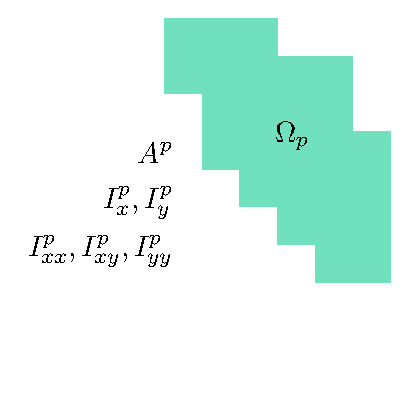
\includegraphics[scale=0.72]{media/om/omp.pdf}
\label{fig:subfigure5}}
\subfigure[Approximating lens $\Omega$]{%
		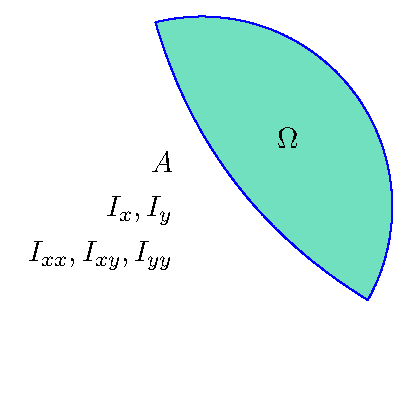
\includegraphics[scale=0.72]{media/om/om.pdf}
\label{fig:subfigure6}}

\caption{Boundary approximation demonstrated in 2D.}
\label{fig:figure3}
\end{figure}

\begin{figure}[h]
	\centering
		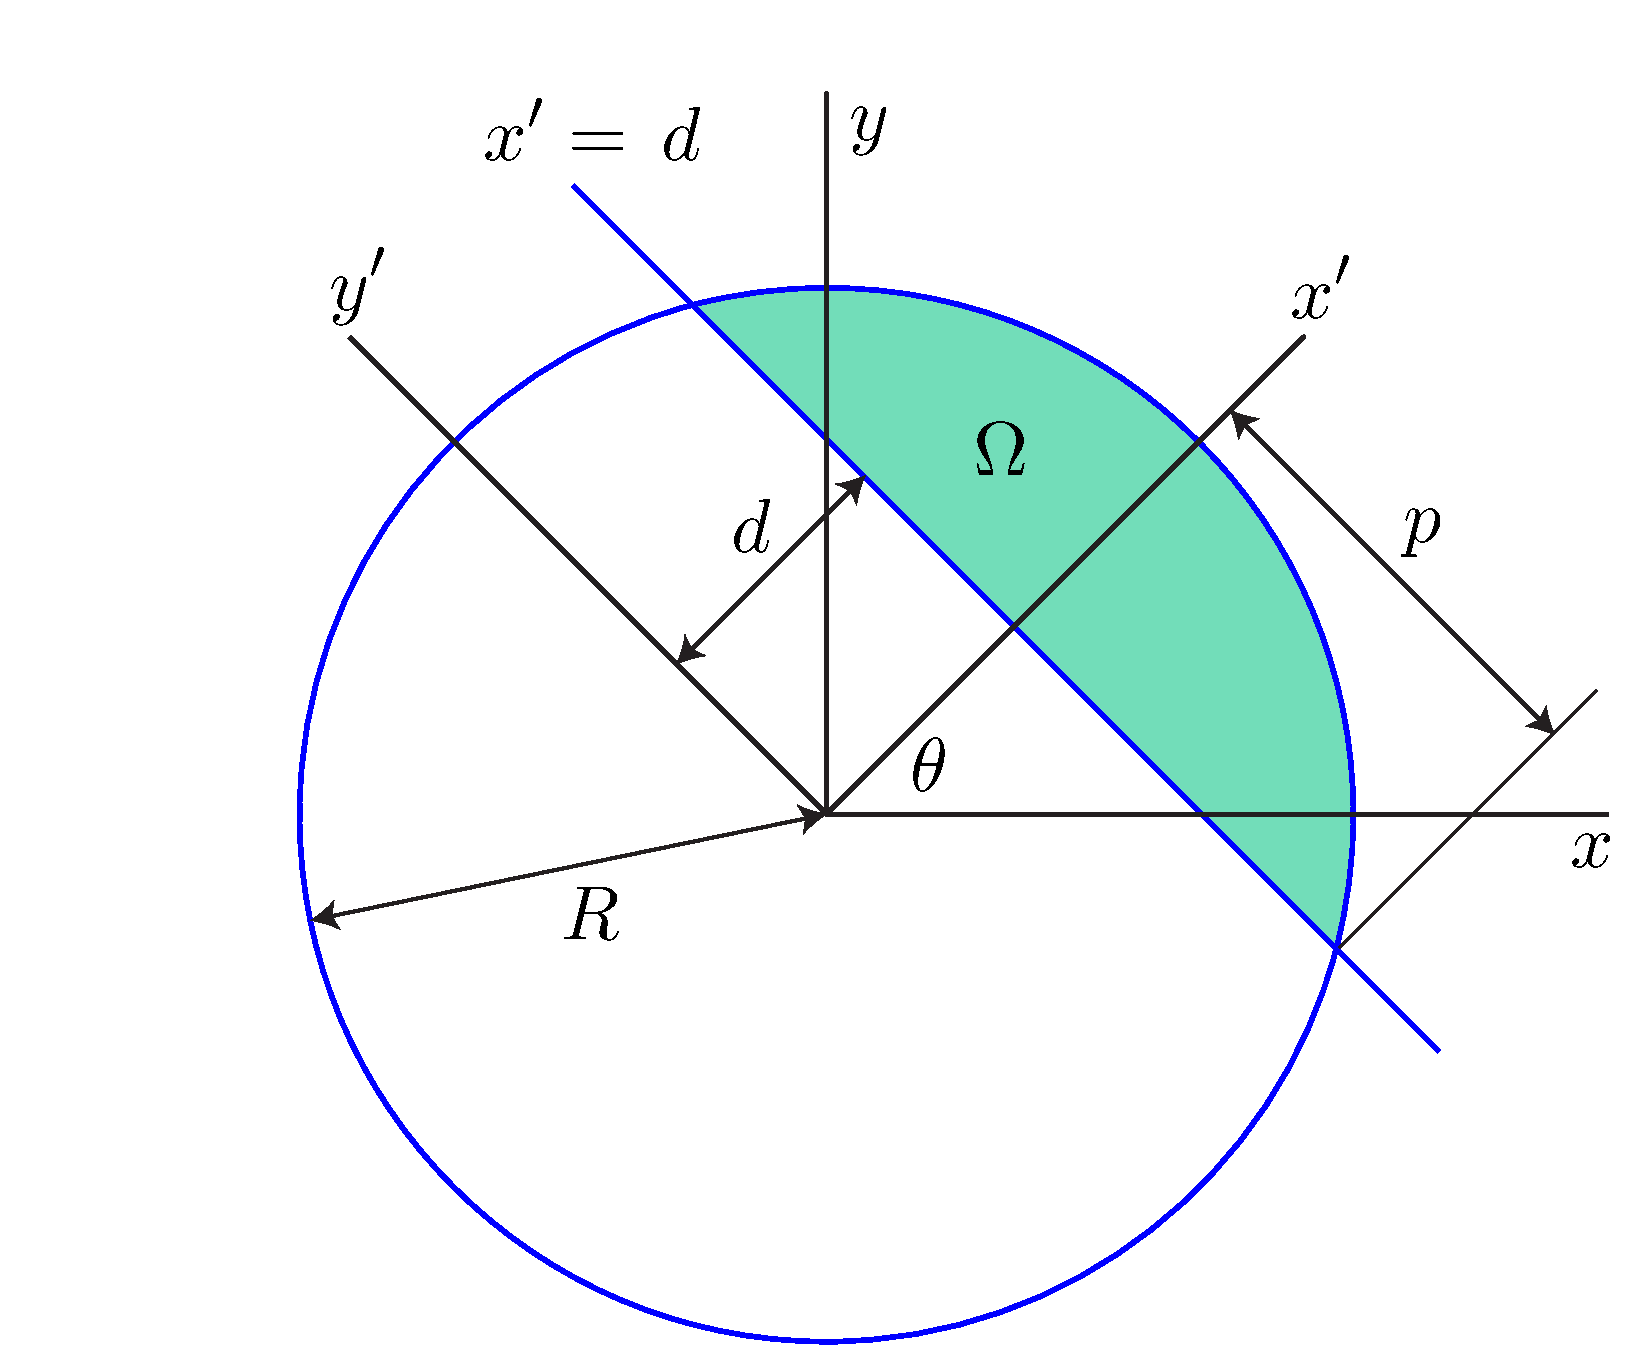
\includegraphics[scale=0.3]{media/om/window.pdf}
	\caption{Plane boundary approximation demonstrated in 2D}
	\label{fig:quad}
\end{figure}
%
\noindent Turning now to the formulation of an error function, we define the following quantities:
\begin{alignat}{3}
f^p &= V^p, \text{\ \ \ \ \ }&&f(d,\psi,\theta) = V, \\
\bm{g}^p &= \left[\begin{array} {ccc} {I_x^p} \\ {I_y^p} \\ {I_z^p} \end{array} \right], \text{\ \ \ \ \ }&&\bm{g}(d,\psi,\theta) = \left[\begin{array} {ccc} {I_x} \\ {I_y} \\ {I_z} \end{array} \right], \\
\bm{h}^p &= \left[\begin{array} {ccc} {I_{xx}^p} & {-I_{xy}^p} & {-I_{xz}^p}\\ {-I_{xy}^p} & {I_{yy}^p} & {-I_{yz}^p} \\ -{I_{xz}^p} & {-I_{yz}^p} & {I_{zz}^p} \end{array} \right],\text{\ \ \ \ \ \ \ }&&\bm{h}(d,\psi,\theta) = \left[\begin{array} {ccc} {I_{xx}} & {-I_{xy}} & {-I_{xz}}\\ {-I_{xy}} & {I_{yy}} & {-I_{yz}} \\ -{I_{xz}} & {-I_{yz}} & {I_{zz}} \end{array} \right].
\end{alignat}
Relative errors in the zeroth, first, and second moments of volume of the window's solid subdomain are then defined as
\begin{align}
e_0(d,\psi,\theta) &=  \sqrt{\frac{(f - f^p)^2}{(f^p)^2}}, \\
e_1(d,\psi,\theta) &=  \sqrt{\frac{(g_i - g_i^p)(g_i - g_i^p)}{g_j^{p}g_j^{p}}}, \\
e_2(d,\psi,\theta) &=  \sqrt{\frac{(h_{ij} - h_{ij}^p)(h_{ij} - h_{ij}^p)}{h_{kl}^{p}h_{kl}^{p}}}.
\end{align}
Finally, we define a single scalar error function as
\begin{align}
\mathcal{F}(d,\psi,\theta) = \beta_0e_0 + \beta_1e_1 + \beta_2e_2,
\end{align}
where $\beta_i$ are adjustable weights in the range $(0,1)$ and $\beta_2 = 1 - \beta_0 - \beta_1$.  The error $\mc{F}$ is an explicit function of the boundary parameters $d$, $\psi$, and $\theta$, where $\psi$ and $\theta$ are the yaw and pitch angles defining the plane and $d$ is the plane's offset from the centroid of the window.  We seek the solution to the following unconstrained minimization problem: $\displaystyle \min_{d, \psi, \theta} \mathcal{F}(d,\psi,\theta)$, which can be solved by a variety of well-established techniques once the moments of volume of $\Omega$ and $\Omega_p$ are defined. \\ \\
%
The moments of volume of $\Omega_p$ are computed based on a straightforward use of voxel dimensions and the parallel axis theorem. The moments of volume of $\Omega$, on the other hand, are computed as a function of $d$ in the primed coordinate system and then are transformed to the original coordinate frame based on $\psi$, and $\theta$. The relevant geometric quantities in the primed system are defined as follows:
\begin{align}
p &= \sqrt{R^2 - d^2}, \\
V^* &= 2\pi\left[-\frac{1}{2}dp^2 + \frac{1}{3}R^3 - \frac{1}{3}(R^2 - p^2)^{3/2} \right], \\
I^*_{x'x'} &= \frac{\pi}{30}\left[-15dp^4 + \sqrt{R^2-p^2}\left(12p^4 - 4p^2R^2 - 8R^4\right) + 8R^5 \right], \\
I^*_{y'y'} &= \frac{\pi}{480}\left[-160d^3p^2 + 128R^5 - \sqrt{R^2-p^2}\left(128R^4 - 96p^2R^2 - 32p^4\right) - 120dp^4 \right],
\end{align}
\begin{align} 
V &=  \begin{cases}
      V^*, & \text{if}\ d \geq 0 \\
      V^* + \frac{4\pi}{3}\left(R^2-p^2\right)^{3/2}, & \text{otherwise}
    \end{cases}\\
I_{x'} &= \frac{\pi}{4}\left[2p^2(R^2-d^2) - p^4 \right],\\
I_{y'} &= I_{z'} = 0, \\
I_{x'y'} &= I_{x'z'} = I_{y'z'} = 0, \\
I_{x'x'} &=  \begin{cases}
      I^*_{x'x'}, & \text{if}\ d \geq 0 \\
       I^*_{x'x'} + \frac{4\pi}{15}(R^2-p^2)^{3/2}(3p^2+2R^2), & \text{otherwise}
    \end{cases} \\
I_{y'y'} &=  \begin{cases}
     I^*_{y'y'}, & \text{if}\ d \geq 0 \\
     I^*_{y'y'} + \frac{2\pi}{15}(R^2-p^2)^{3/2}(p^2+4R^2), & \text{otherwise}
    \end{cases} \\
I_{z'z'} &= I_{y'y'}.
\end{align}
Unsurprisingly, certain moments of volume exhibit symmetries in regard to the $y'$ and $z'$ axes. \\ \\
%
The geometric quantities are then transformed back to the original desired coordinate frame. This transformation is different for the zeroth, first, and second moments of volume due to the different tensor rank for each of these quantities. Once the moments of volume of $\Omega$ have been transformed to the original coordinate frame, they can be compared to those of $\Omega_p$. The first and second moments of volume are transformed in the following manner (no transformation is required for the zeroth moment of volume):
\begin{gather}
\bm{R} = \left[\begin{array} {ccc} {\cos\psi\cos\theta} & {-\sin\psi} & {\cos\psi\sin\theta}\\ {\sin\psi\cos\theta} & {\cos\psi} & {\sin\psi\sin\theta}, \\
{-\sin\theta} & {0} & {\cos\theta}\end{array} \right], \\
\left[\begin{array} {ccc} {I_x} \\ {I_y} \\ {I_z} \end{array} \right] = \bm{R} \left[\begin{array} {ccc} {I_{x'}} \\ {I_{y'}} \\ {I_{z'}} \end{array} \right],
\end{gather}
\begin{gather}
\bm{I}' = \left[\begin{array} {ccc} {I_{x'x'}} & {-I_{x'y'}} & {-I_{x'z'}}\\ {-I_{x'y'}} & {I_{y'y'}} & {-I_{y'z'}} \\ -{I_{x'z'}} & {-I_{y'z'}} & {I_{z'z'}} \end{array} \right], \\
\bm{I} = \left[\begin{array} {ccc} {I_{xx}} & {-I_{xy}} & {-I_{xz}}\\ {-I_{xy}} & {I_{yy}} & {-I_{yz}} \\ -{I_{xz}} & {-I_{yz}} & {I_{zz}} \end{array} \right] = \bm{R}\bm{I}'\mathbf{R}^T.
\end{gather}
\noindent With all relevant quantities defined, the \textit{subplex search method}~\cite{rowan} is used to minimize the error function using an implementation in the package \textit{NLopt}~\cite{nlo}. The method is a \textit{derivative-free} method that is well suited for optimizing objective functions that are noisy or discontinuous. It was selected as the optimization approach due to the existence of square roots in the objective function, and the fact that robustness to a variety of inputs was the highest priority in developing the algorithm. A convergence tolerance $\varepsilon$ is defined such that on successive iterations, $\left| \mathcal{F}_{k+1} - \mathcal{F}_{k}\right| < \varepsilon$, where $k$ is the iteration number. \\ \\
%
For the specific examples and algorithm parameters discussed later in this chapter, convergence is achieved for each boundary approximation after typically hundreds of iterations. This large value may be due to the admittedly tight tolerance value for $\varepsilon$ of $10^{-14}$, to nonlinearities or saddle points in the error function, or to inefficiencies in the nonlinear optimization tool used. However, because the point cloud generation step generates good results, and the entire process usually completes in less than one minute of wall clock time on a personal computer even for complex geometries, the convergence rate was not further explored as a means of improving the algorithm. \\ \\
%
Finally, the solution is only accepted if the error function is below a specified value $\overline{\mathcal{F}}$, i.e., $\Omega$ approximates $\Omega_p$ to a satisfactory degree. Specifically, we require that once convergence has been satisfied, the criterion $\mathcal{F} < \overline{\mathcal{F}}$ must also be met for the point and normal to be retained. In this way, outlier points for which the error minimization performs poorly are discarded. This typically occurs in regions of high curvature, where a plane does not approximate such a boundary well. The point cloud is dense enough that simply discarding these points does not cause any discernible amount of under-sampling of the surface. \\ \\
%
The solution to the minimization problem yields the values $d$, $\psi$, and $\theta$ that determine the optimal surface $\mathcal{S}$, from which the boundary point and normal are defined. Refer to~\tabref{surface} for a summary of variables used in approximating the boundary.

\begin{table}[]
 \centering
   \begin{tabular}{|c||c|}
   \hline
   {\textbf{Variable}} & {\textbf{Description}} \\ \hline \hline
   $\mathcal{D}$ & approximating sphere to $\mathcal{W}$ \\ \hline
   $\mathcal{S}$ & approximating surface to boundary of interest \\ \hline      
   $R$ & radius of $\mathcal{D}$ \\ \hline   
   $\Omega_p$ & physical space covered by voxels belonging to $\mathcal{W}$ \\ \hline
   $\Omega$ & physical space covered by approximating lens of $\Omega_p$ \\ \hline      
   $(x,y,z)$ & axes aligned with image directions, whose origin is at the center of $\mathcal{W}$\\ \hline
   {$(x',y',z')$} & axes $(x,y,z)$ transformed such that $x'$ passes through centroid of $\Omega$ \\ \hline
%   {} & where $x'$ passes through the centroid of $\Omega$ \\ \hline   
   $d$ & perpendicular distance from center of $\mathcal{D}$ to plane $\mathcal{S}$  \\ \hline
   $\psi$ & yaw angle of rotation between $(x,y,z)$ and $(x',y',z')$ axes \\ \hline   
   $\theta$ & pitch angle of rotation between $(x,y,z)$ and $(x',y',z')$ axes \\ \hline
   $V^p$ & volume of $\Omega_p$ \\ \hline
   $I_{x}^p, I_y^p$ & first moments of volume of $\Omega_p$ \\ \hline     
   $I_{xy}^p, I_{xz}^p, I_{yz}^p$ & products of volume of $\Omega_p$ \\ \hline      
   $I_{xx}^p, I_{xy}^p, I_{yy}^p$ & second moments of volume of $\Omega_p$ \\ \hline
   $V$ & volume of $\Omega$ \\ \hline
   $I_{x}, I_y$ & first moments of volume of $\Omega$ \\ \hline
   $I_{xy}, I_{xz}, I_{yz}$ & products of volume of $\Omega$ \\ \hline   
   $I_{xx}, I_{xy}, I_{yy}$ & second moments of volume of $\Omega$ \\ \hline
   $e_0$ & relative error in zeroth moment of volume \\ \hline
   $e_1$ & relative error in first moment of volume \\ \hline
   $e_2$ & relative error in second moment of volume \\ \hline   
   $\beta_0$ & weighting coefficient for zeroth moment of volume error \\ \hline
   $\beta_1$ & weighting coefficient for first moment of volume error \\ \hline
   $\beta_2$ & weighting coefficient for second moment of volume error \\ \hline 
   $\varepsilon$ & convergence tolerance for minimization of function $\mathcal{F}$ \\ \hline
   $\overline{\mathcal{F}}$ \rule{0mm}{4mm} & largest acceptable value of function $\mathcal{F}$ \\ \hline        
\end{tabular}
\caption{List of variables for boundary approximation}
\label{tab:surface}
\end{table}

\subsubsection{Boundary Point and Normal Placement}

Once the parameters $d$, $\psi$, and $\theta$ are selected to fully define the surface that approximates the boundary, a point location and outward normal are determined. The outward pointing normal is defined from the transformation of the $x$ axis to the $x'$ axis, i.e., the first column of matrix $\bm{R}$, and thus defined as such: $\bm{n} = -(\cos\psi\cos\theta,\text{\ }\sin\psi\cos\theta,\text{\ }-\sin\theta)$. With the origin at the center of sphere $\mathcal{D}$, the location of the boundary normal is then simply $\mathbf{x}_p = -d\bm{n}$.

%%%%%%%%%%%%%%%%%%%%%%%%%%%%%%%%%%%%%%%%%%%%%%%
%%%%%%%%%%%%%%%%%%%%%%%%%%%%%%%%%%%%%%%%%%%%%%%
\subsection{Surface Reconstruction}
\label{Surface Reconstruction}

Surface reconstruction is the process of generating closed, manifold, polygonized surfaces from point clouds. The research found in the literature typically expects a dense, noisy population of points that are generated from laser-based scanners. The proposed algorithm does not in general produce a point cloud as dense as do laser scanners, but a brief review of surface reconstruction techniques is still informative. \\ \\
%
Among the most well-known surface reconstruction algorithms are the \textit{Power Crust} and \textit{Poisson surface reconstruction} techniques. Amenta \textit{et al.}~\cite{amenta_2001} presented the \textit{Power Crust} algorithm for reconstructing watertight surfaces from unoriented point clouds. It first constructs the \textit{medial axis transform} from the point cloud, which is the set of maximal balls completely contained in the interior of the surface. The algorithm then applies an inverse transform to approximate the medial axis and produce a piecewise-linear surface. The algorithm does not perform well when the point set is not sufficiently dense. Kazhdan \textit{et al.} presented \textit{Poisson surface reconstruction}~\cite{kazhdan_2008} and subsequently \textit{screened Poisson surface reconstruction}~\cite{kazhdan_2013} for oriented point clouds. They compute an indicator function defined as 1 for points inside the surface and 0 for points outside, whose gradient approximates the vector field defined by the oriented point cloud. This amounts to solving a Poisson problem for an implicit indicator function, followed by application of marching cubes to polygonize the surface. The \textit{screened} approach provides a soft constraint that encourages the reconstructed isosurface to pass through the input points. In practice, the screened approach is significantly more robust than the original approach in generating manifold surfaces from complex point clouds. The technique produces smooth surfaces that exhibit a resiliency to noise, outliers, and under-sampling that makes it arguably best-in-class. \\ \\
%
Many other surface reconstruction approaches exist, including those making use of moving least squares, Delaunay and Voronoi constructions, and variational approaches~\cite{berger}. A novel Voronoi-based approach is presented as an alternative to these approaches that is tuned to address the type of noise and point density from the point cloud generation algorithm from the previous section. \\ \\
%
The proposed surface reconstruction technique relies on constructing a \textit{Voronoi diagram}, which for our purposes is a nearest neighbor partitioning of $\mathbb{R}^3$ based on a set of input \textit{Voronoi sites}. The desired output from a Voronoi partition is a mesh - namely, a set of points, edges, facets, and cells (and their connectivities) that discretize space. Define a half-space $D(\bm{p},\bm{q})$ comprising all points $\bm{x}$ as close, or closer, to site $\bm{p}$ than to site $\bm{q}$:
\begin{equation}
D(\bm{p},\bm{q}) = \{\bm{x} \mid d(\bm{p},\bm{x}) \leq d(\bm{q},\bm{x})\},
\end{equation}
where a distance function $d$ must be defined. Although there are instances of more exotic distance functions leading to modified Voronoi approaches, the distance function for standard Voronoi diagrams is simply the Euclidean distance. The \textit{Voronoi cell} $V(\bm{p})$ associated with site $\bm{p}$ is the intersection of all half-spaces involving site $\bm{p}$ and all other sites $\bm{q}$ belong to the set $\mathcal{P}$:
\begin{equation}
V(\bm{p}) = \bigcap \limits_{\bm{q} \in \mathcal{P}, \bm{q} \neq \bm{p}} D(\bm{p},\bm{q}).
\end{equation}
A number of important properties exist for Voronoi partitions and their dual \textit{Delaunay tessellations}. For these purposes, though, the most important property is that the surface extracted from a set of Voronoi cells connected by shared facets is watertight and manifold. Several important considerations must be made in constructing a Voronoi partition, including degenerate and near-degenerate cases, the data schema and order of construction of the connected polytopes, and the
performance of the algorithm. Refer to Aurenhammer~\cite{aurenhammer_1991} for a detailed survey of the mathematical and algorithmic approaches to Voronoi diagrams. \\ \\
%
The proposed technique involves the following steps, to be described in turn:
\begin{itemize}[noitemsep]
\item Generate Voronoi site set from oriented point cloud and perform Voronoi partition of image
\item Define b-rep as the set of facets that share Voronoi sites with different material types, and perform cleanup on that surface
\item \textit{Decimate} (coarsen) the surface to a more tractable mesh resolution
\end{itemize}

\subsubsection{Voronoi Site Generation and Voronoi Partitioning}

Given the location of a boundary point $\bm{x}_p$ and orientation of its corresponding normal $\bm{n}$, two Voronoi sites are placed on either side of the point along the line of action of the normal, as shown in~\figref{vor4} and~\figref{d2dvor3}. They are separated from the point by a distance $b$, and thus their locations are $\bm{x}_p \pm b \bm{n}$. The two Voronoi sites are assigned material types. For the two-material case considered here, the site corresponding to the position $\bm{x}_p - b\bm{n}$ is inside $\Omega$, and thus is assigned material $m$. The site corresponding to the position $\bm{x}_p + b\bm{n}$ is outside $\Omega$, and thus is assigned a void material. \textit{Voronoi partitioning} is performed using an implementation from \textit{Qhull}~\cite{barber_1996}, that is robust even for near-degenerate Voronoi site locations. The sequence of point cloud generation, Voronoi site placement, and Voronoi partitioning is demonstrated in~\figref{d2dvor}.

\begin{figure}[htbp!]
\centering
\subfigure[]{%
		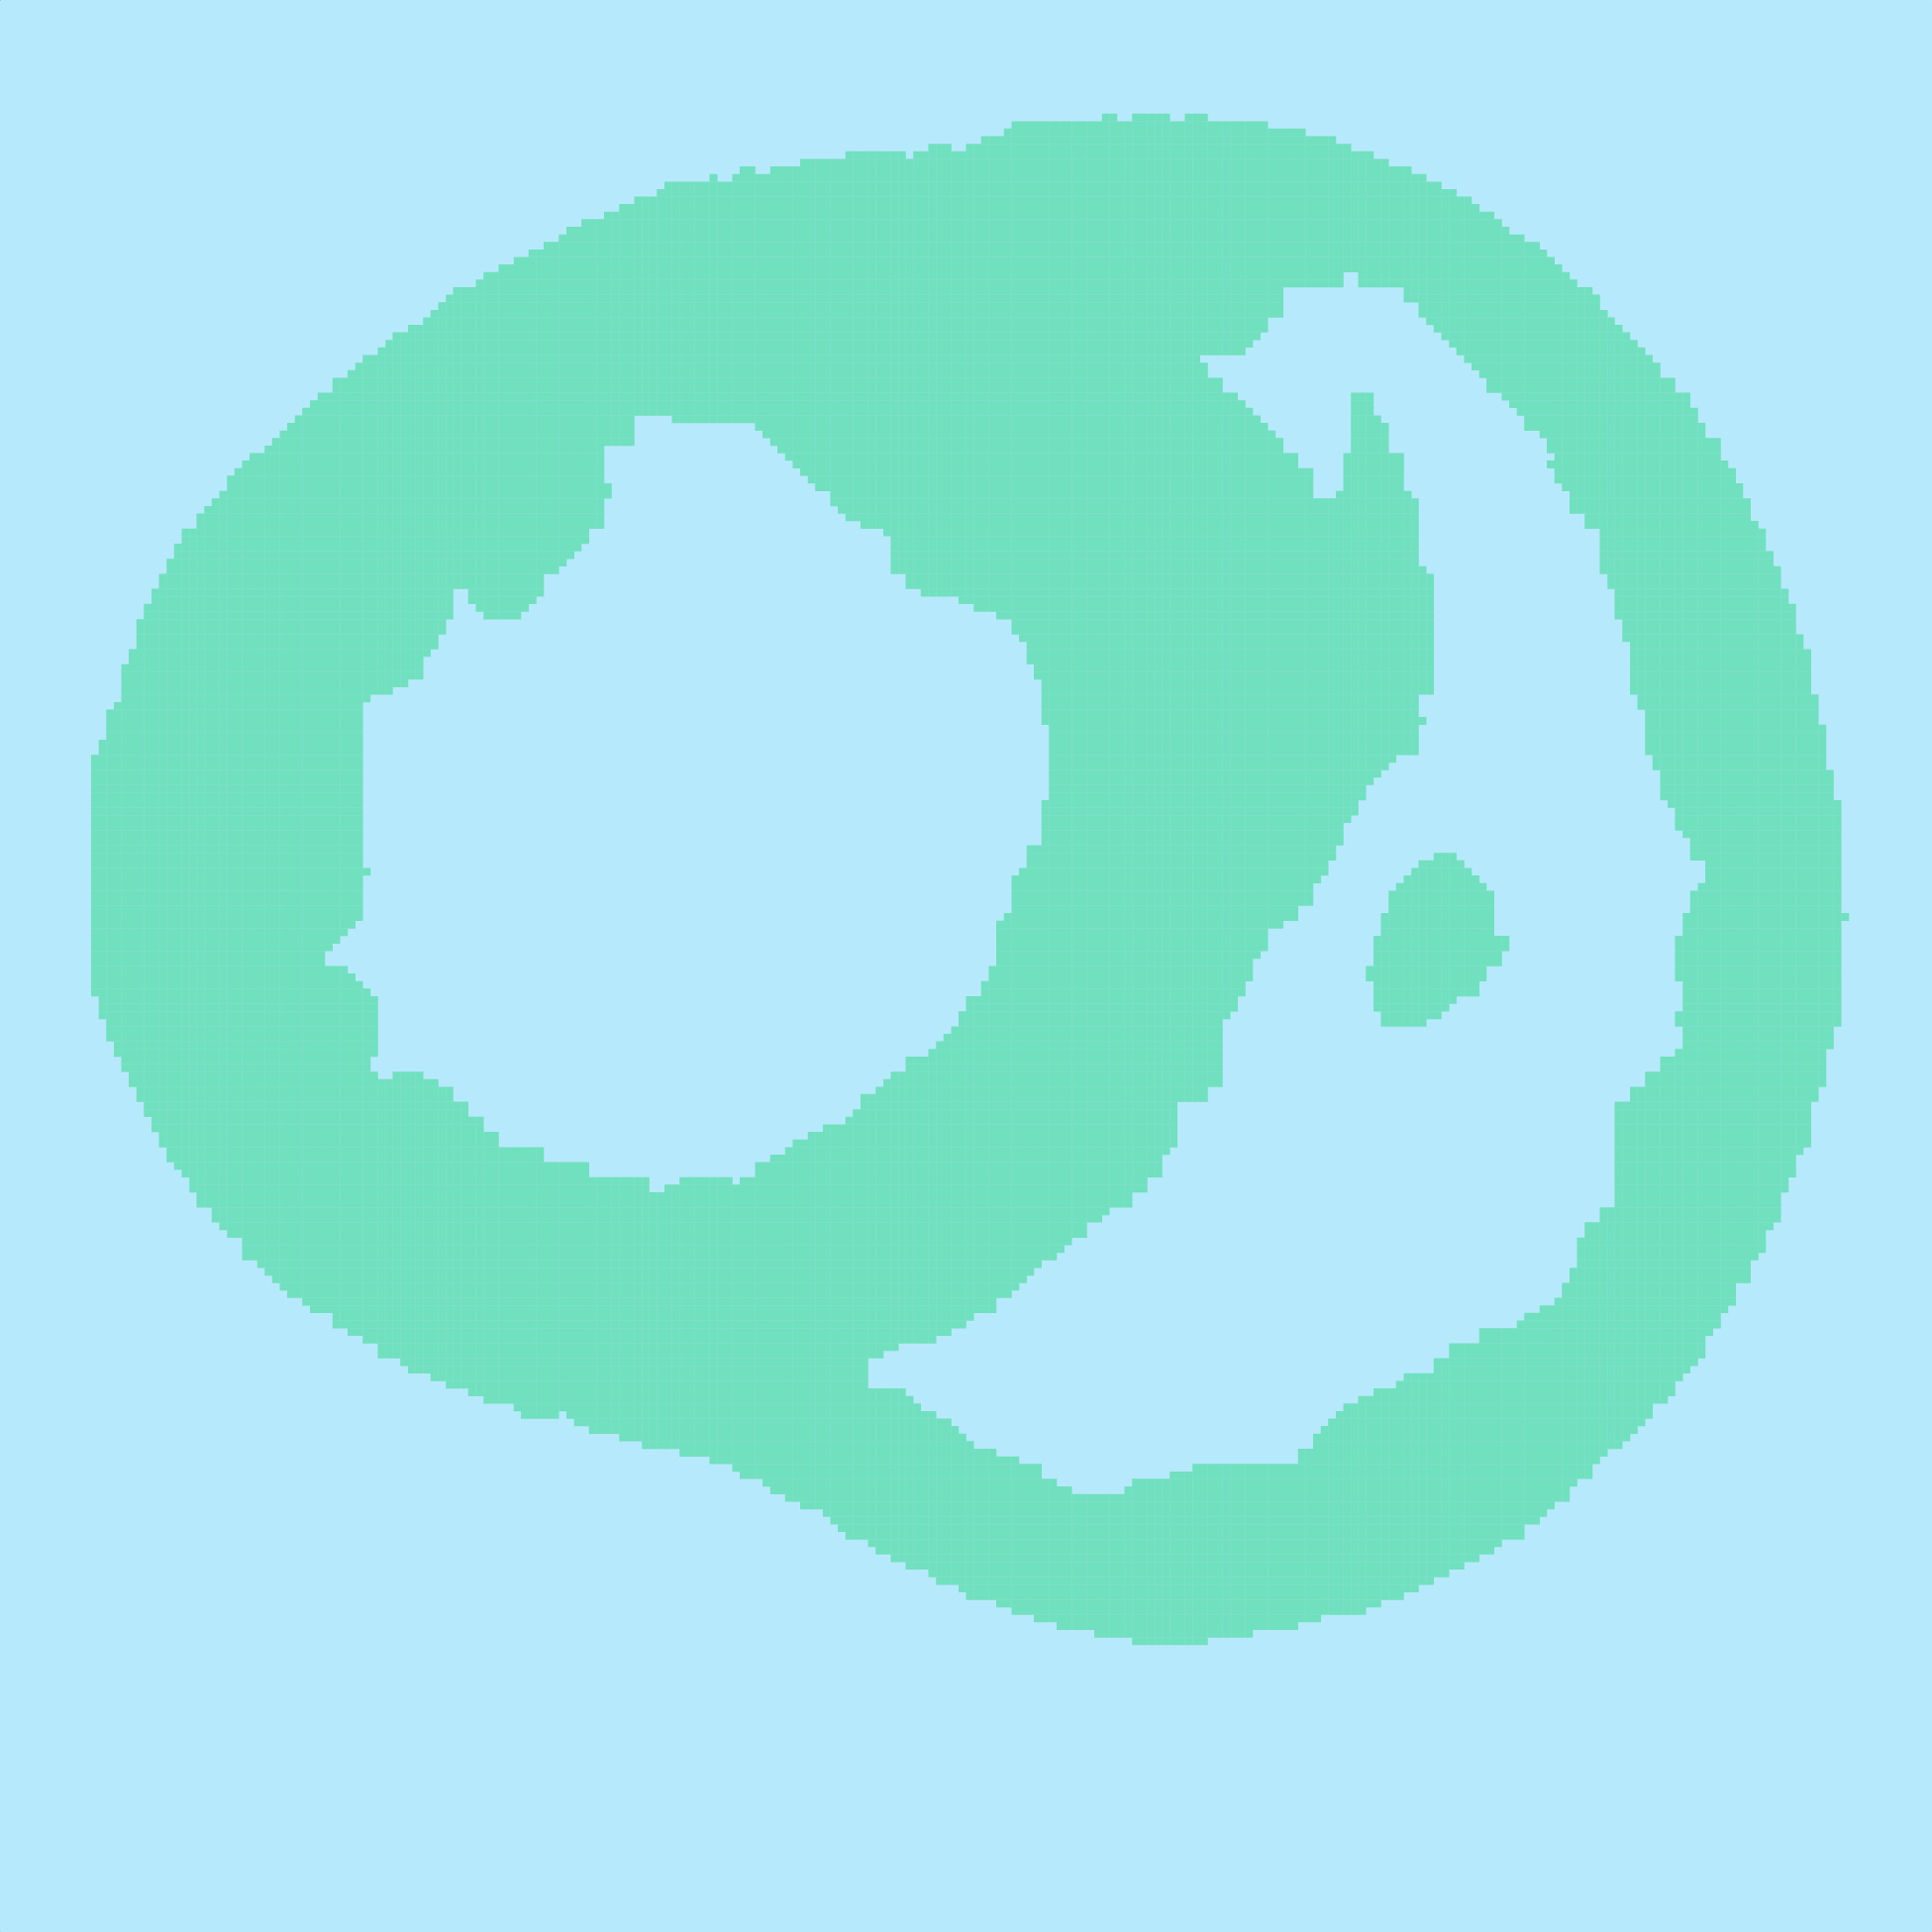
\includegraphics[scale=0.33]{media/vv/a1.png}
\label{fig:d2dvor1}}
\subfigure[]{%
		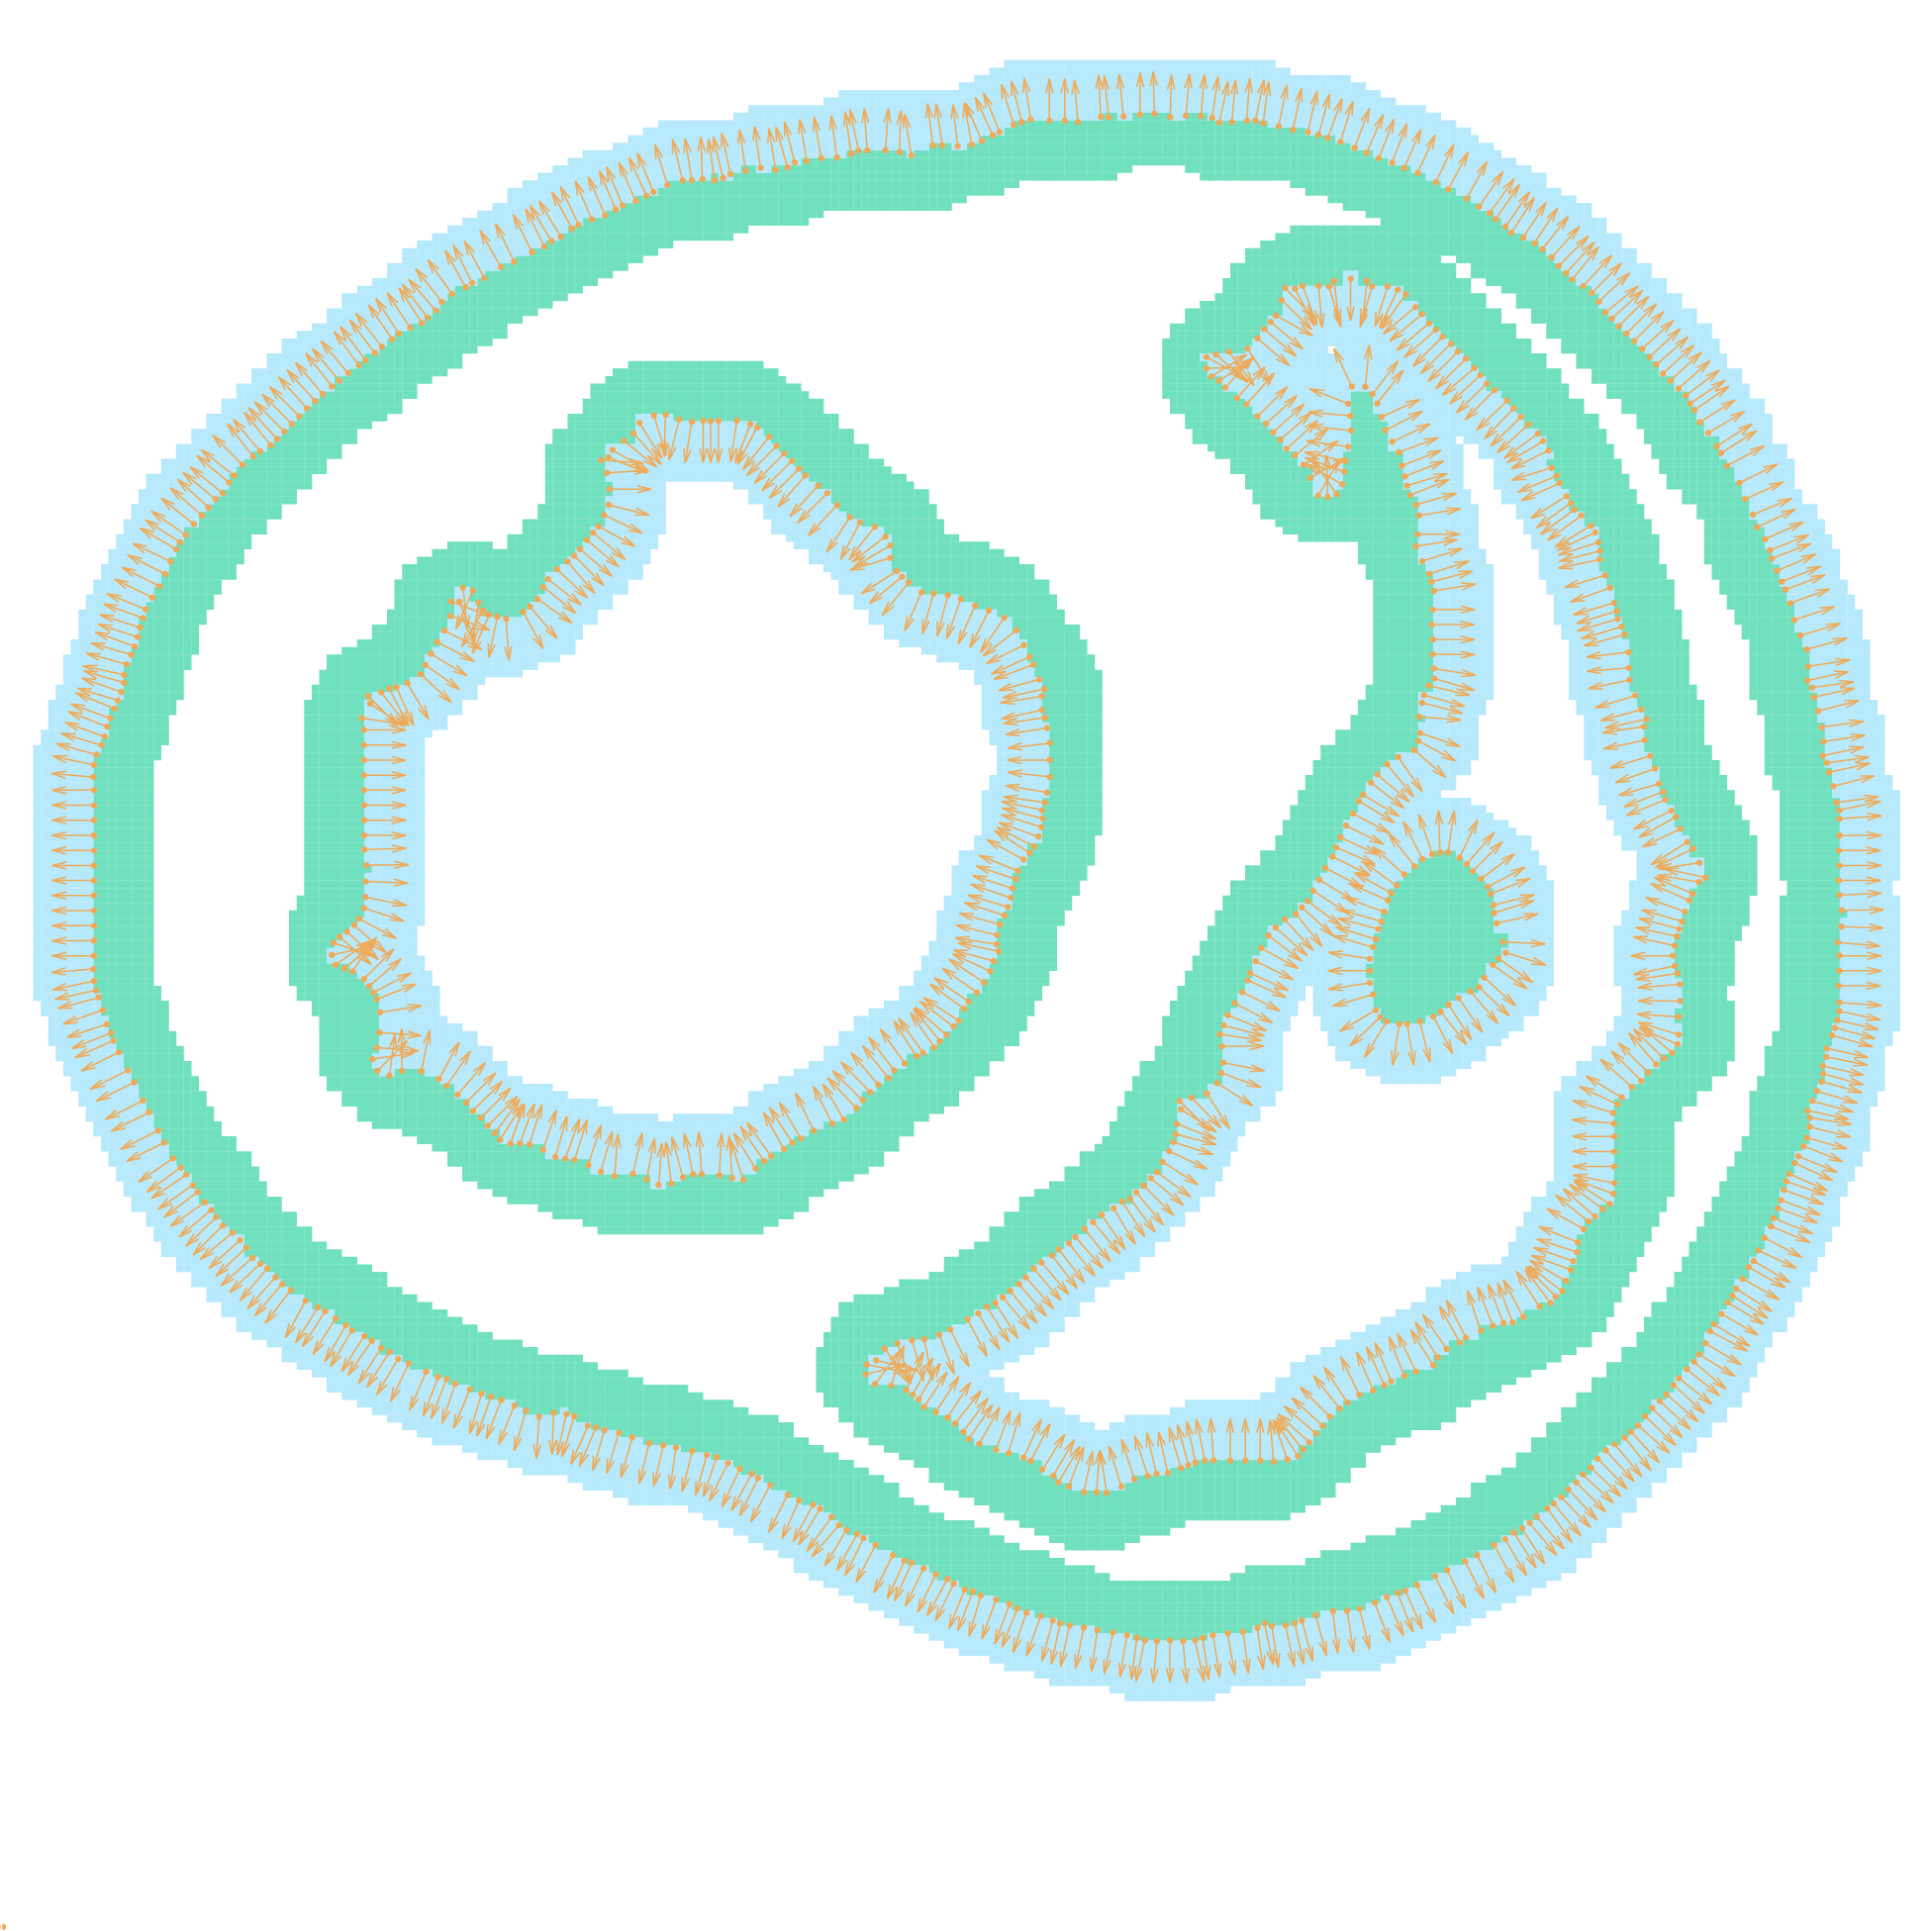
\includegraphics[scale=0.33]{media/vv/a2.png}
\label{fig:d2dvor2}}
\subfigure[]{%
		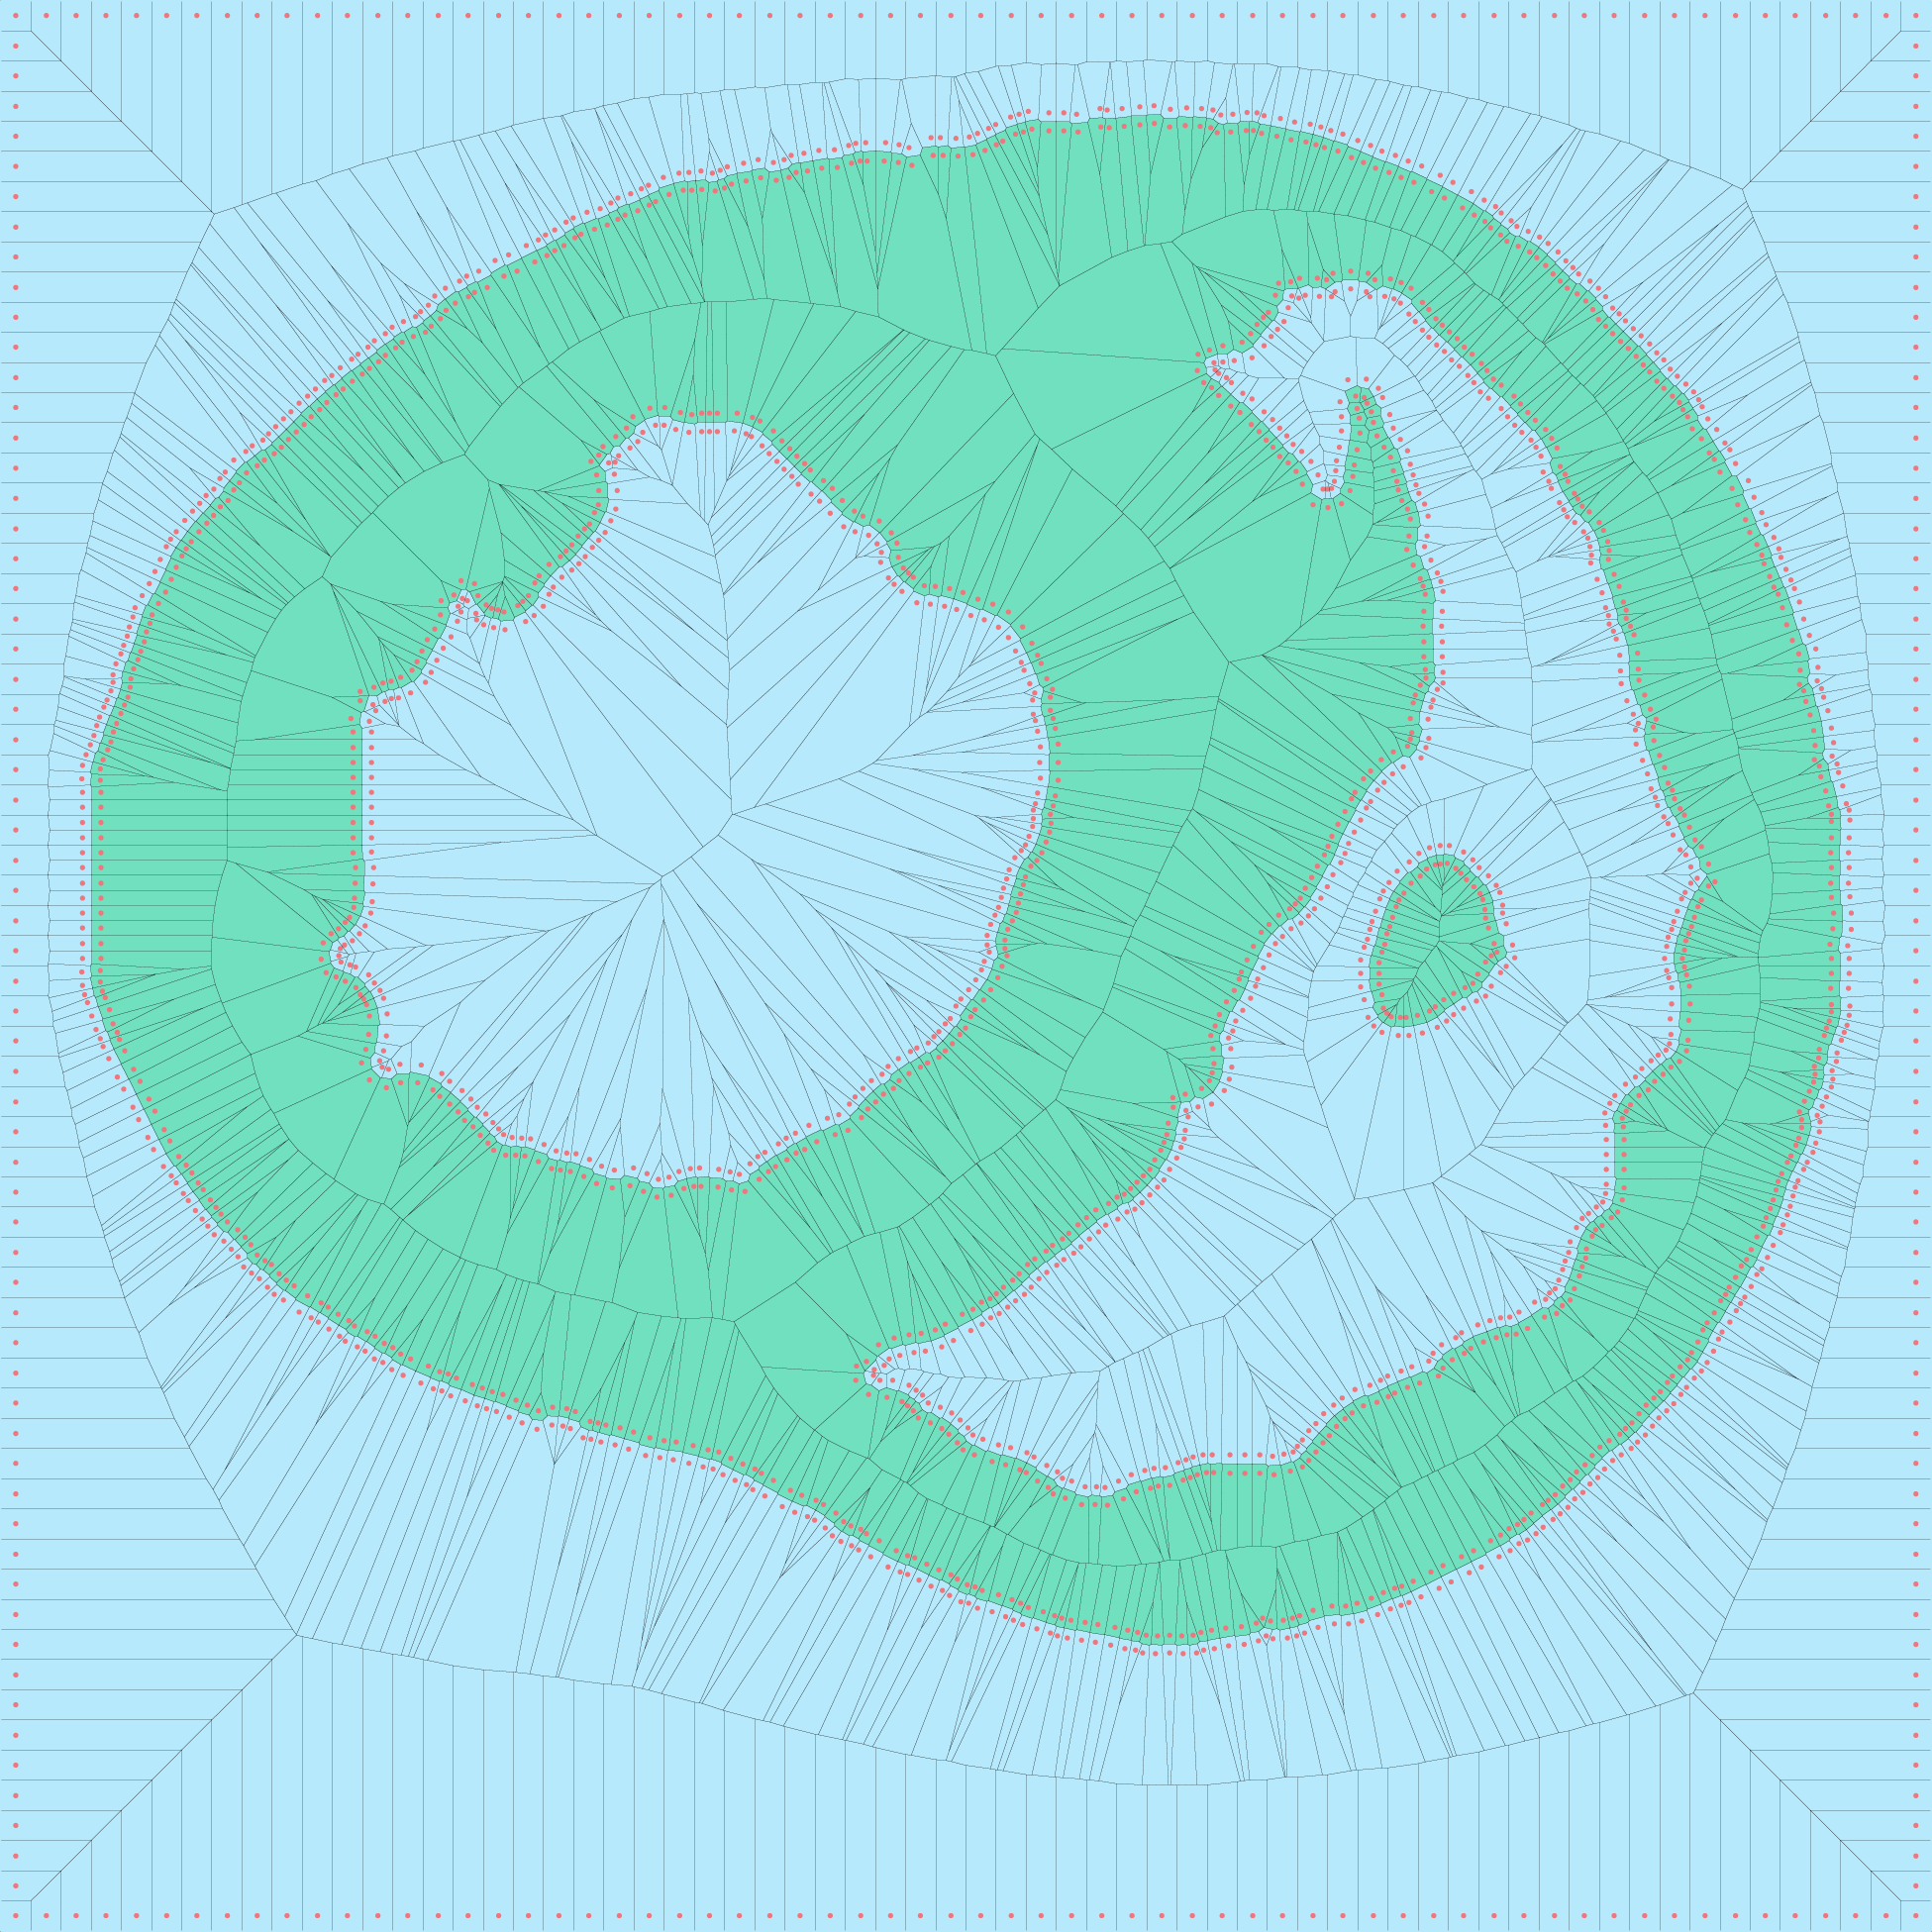
\includegraphics[scale=0.33]{media/vv/a3.png}
\label{fig:d2dvor3}}
%\subfigure[]{%
%		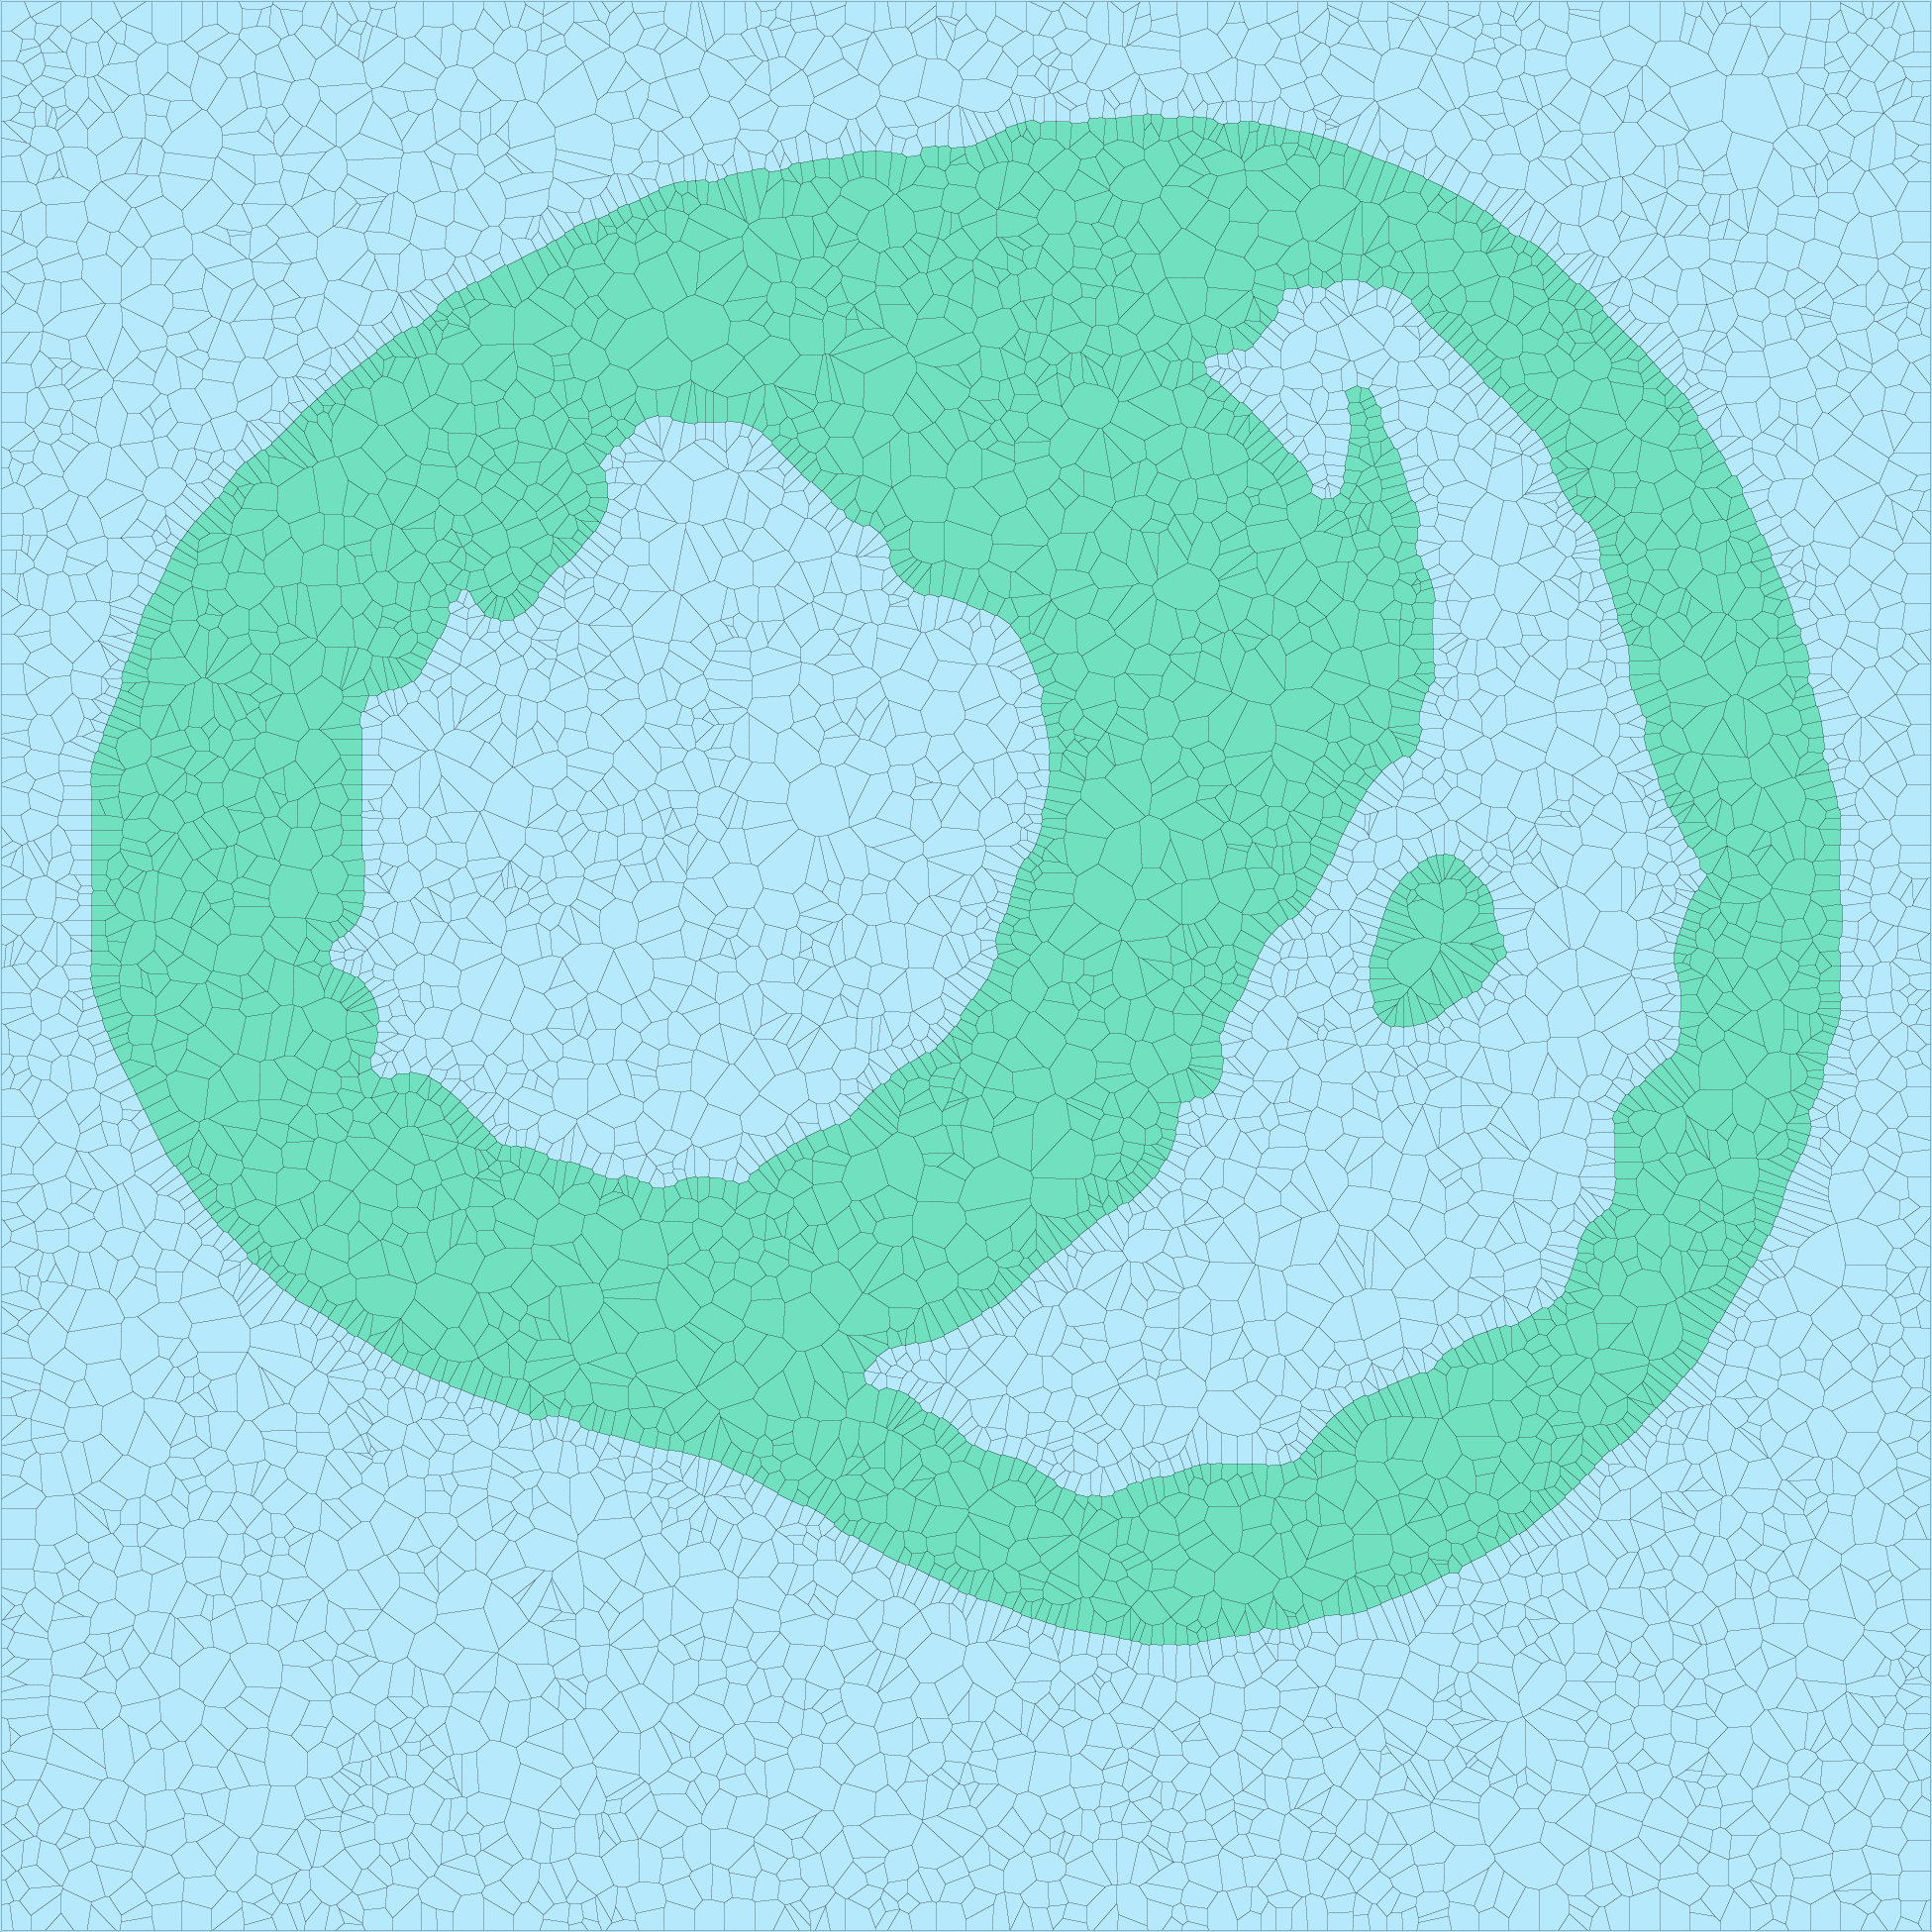
\includegraphics[scale=0.4]{media/vv/a4.png}
%\label{fig:d2dvor4}}
%
\caption{(a) Segmented image of 2D slice of \textit{ex vivo} canine heart (image mask generated from MRI data from Cardiovascular Research Grid~\cite{cvgg}), (b) resulting point cloud, and (c) Voronoi site placement and subsequent Voronoi partitioning and surface extraction.}
\label{fig:d2dvor}
\end{figure}

\subsubsection{Surface Extraction and Cleanup}

The b-rep is extracted from the Voronoi partition as the set of facets that share Voronoi sites of differing material types. An additional step is performed, however, to mitigate undesired ``cross-talk'' facets caused by Voronoi partitioning of neighboring site pairs. ``Good facets'' are identified as those b-rep facets whose Voronoi sites belong to a site pair originating from the same point and normal, and ``bad facets'' are those b-rep facets whose Voronoi sites originate from different points in the point cloud. For surfaces with small curvature, the area of good facets significantly outweighs that of the bad facets. Nonetheless, the existence of bad facets causes a stair-stepping feature in the resulting surface that is unacceptable. \\ \\
%
The artifact is addressed as follows: ``bad edges'' are identified as those edges that share two bad facets. Networks of connected bad edges are identified, and each network is collapsed to one point (see \figref{cross1}). For surfaces with a small amount of curvature, no bad edges are connected, and thus each is independently collapsed. Any good facet that is connected to a network of bad edges is modified to connect to the new collapsed point. The good facets are triangulated to maintain planarity following the removal of bad facets. This increases the data required to define the surface mesh, but the decimation step described in the next section resolves this issue immediately. The sequence is demonstrated for an \textit{ex vivo} heart example in~\figref{cross2}. \\

\begin{figure}[htbp!]
\centering
\subfigure[]{%
		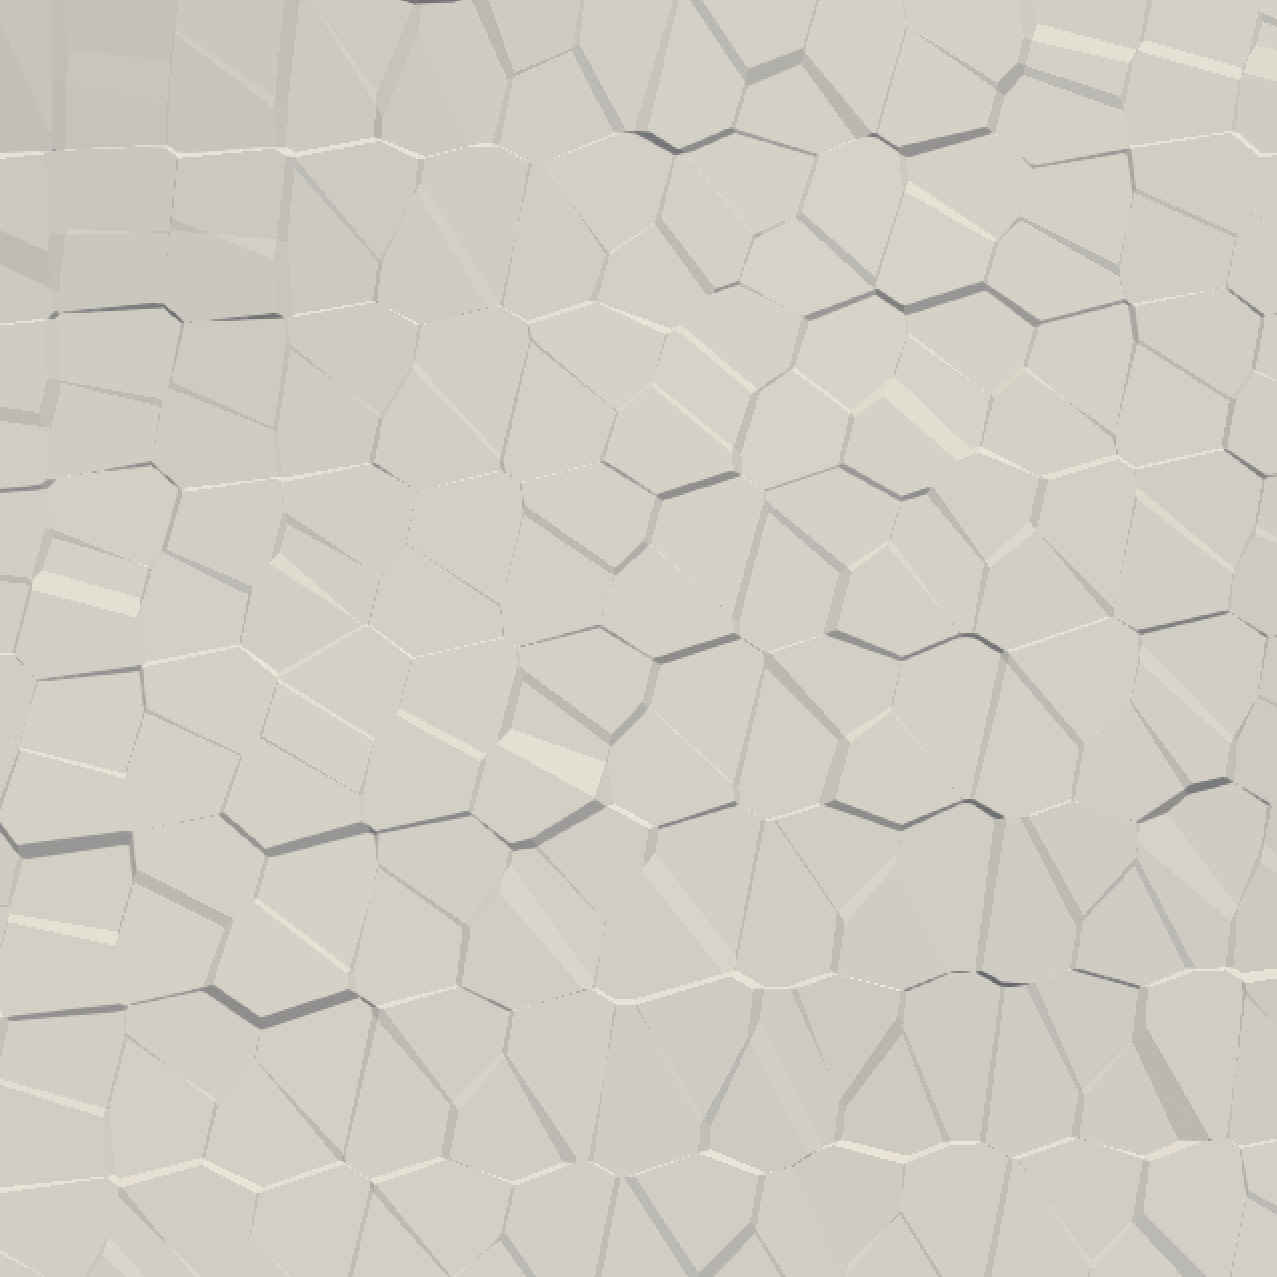
\includegraphics[scale=0.09]{media/2-shabaka/3-clean-zoom/1-init-zoom.png}
\label{fig:cross1-1}}	
\subfigure[]{%
		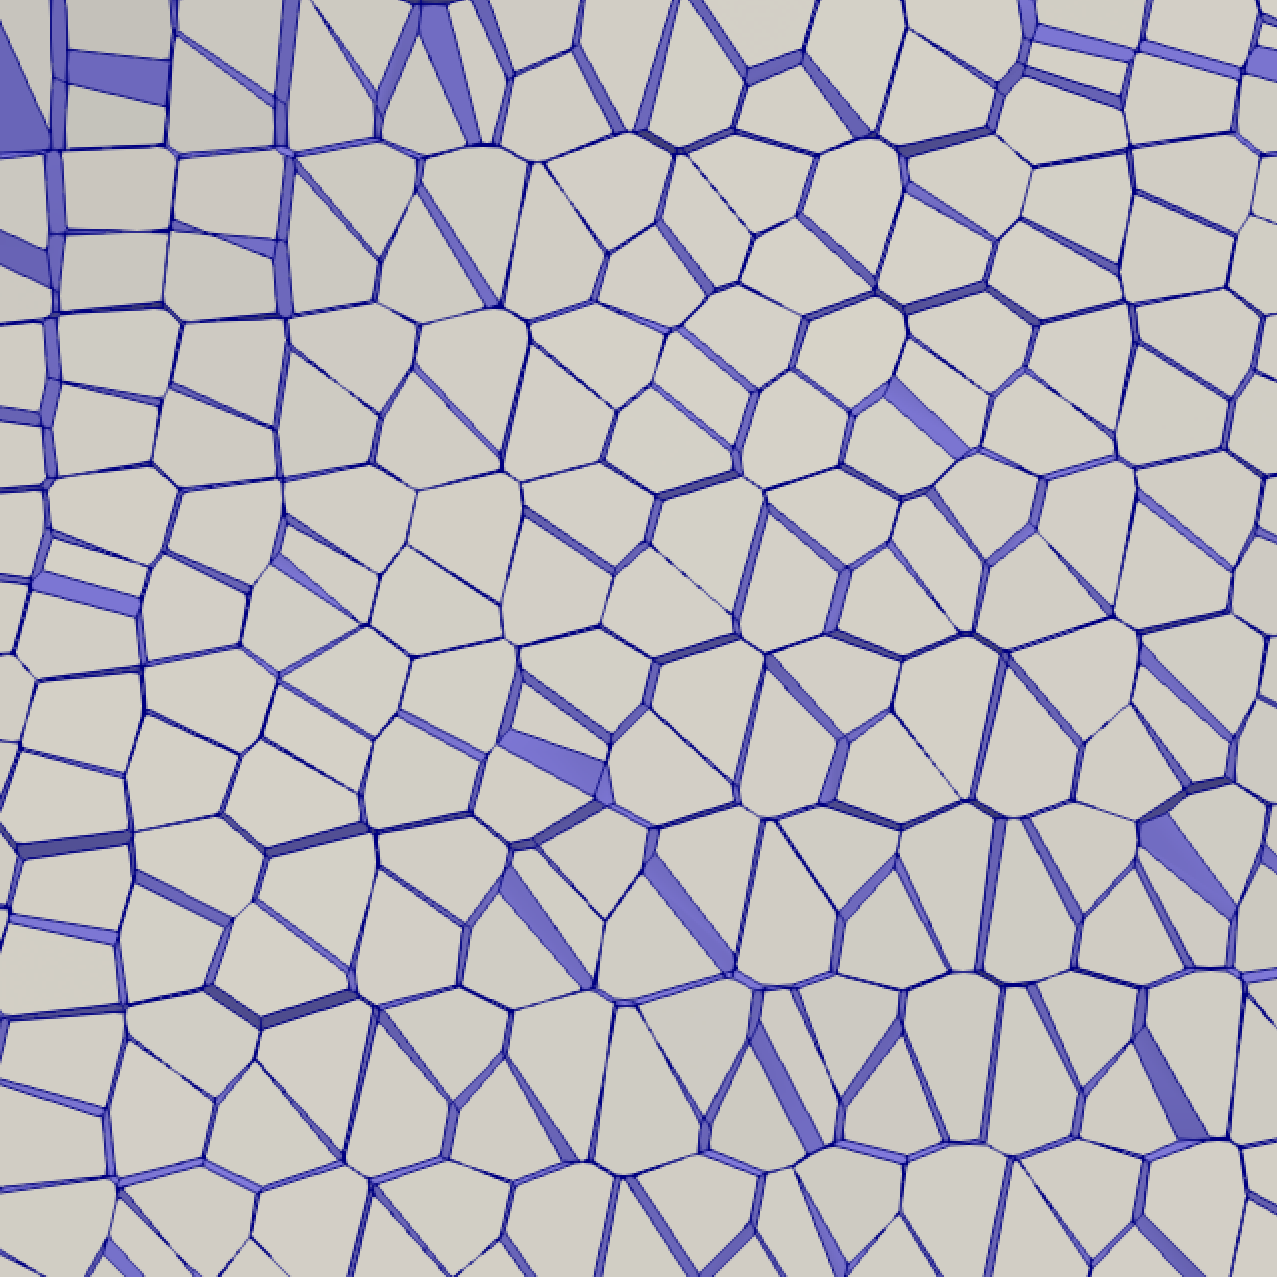
\includegraphics[scale=0.09]{media/2-shabaka/3-clean-zoom/2-badfacets-zoom.png}
\label{fig:cross1-2}}
\subfigure[]{%
		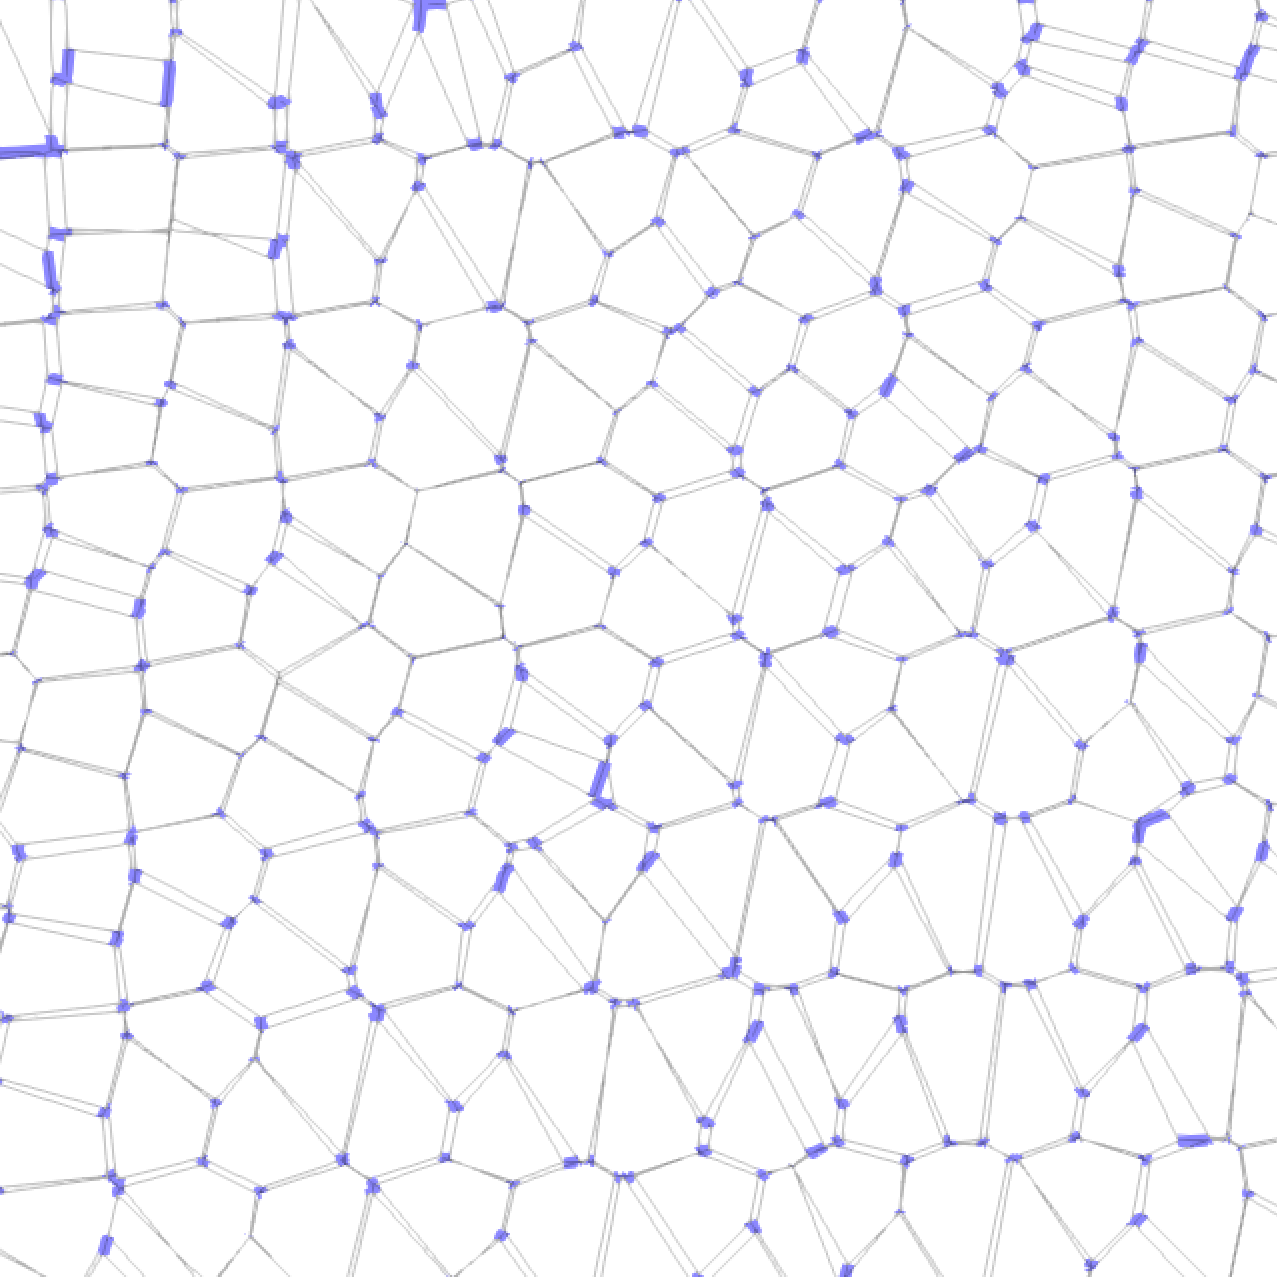
\includegraphics[scale=0.09]{media/2-shabaka/3-clean-zoom/3-badsegs-zoom.png}		
\label{fig:cross1-3}}
\subfigure[]{%
		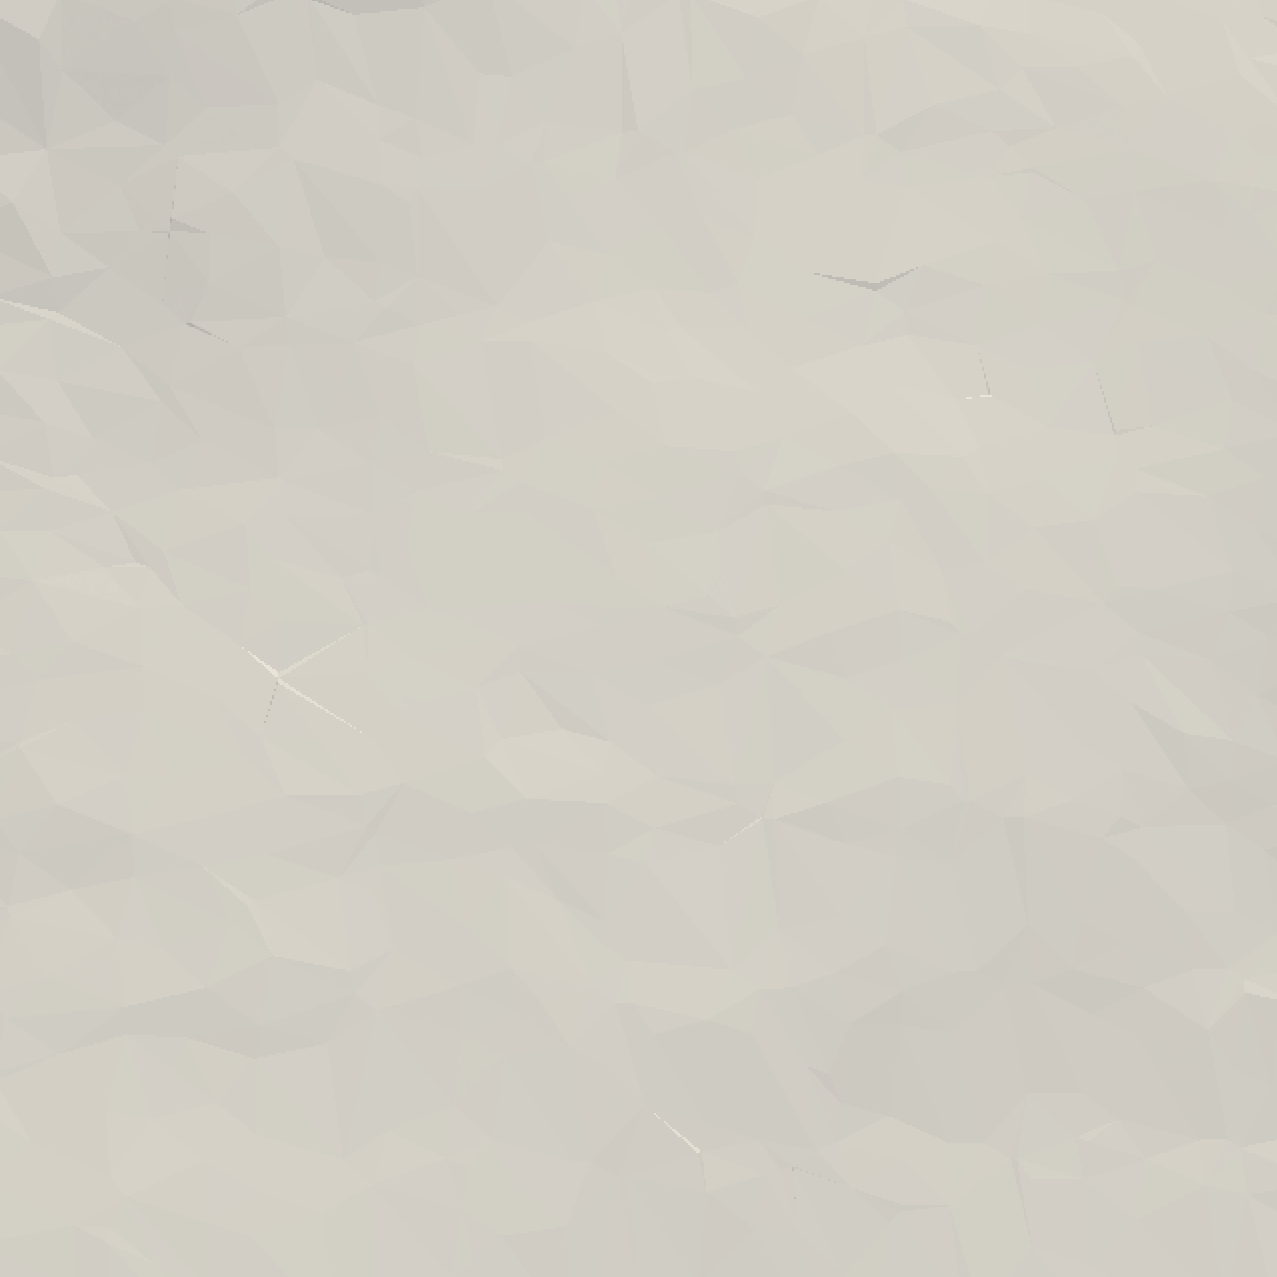
\includegraphics[scale=0.09]{media/2-shabaka/3-clean-zoom/4-fine-zoom.png}
\label{fig:cross1-4}}				
%
\caption{Cleanup of undesirable ``cross-talk'' facets for a surface patch: (a) initial surface following Voronoi-based surface reconstruction, (b) identification of ``cross-talk'' facets, (c) identification of edges to be collapsed, (d) final cleaned surface}
\label{fig:cross1}
\end{figure}

\begin{figure}[htbp!]
\centering
\subfigure[]{%
		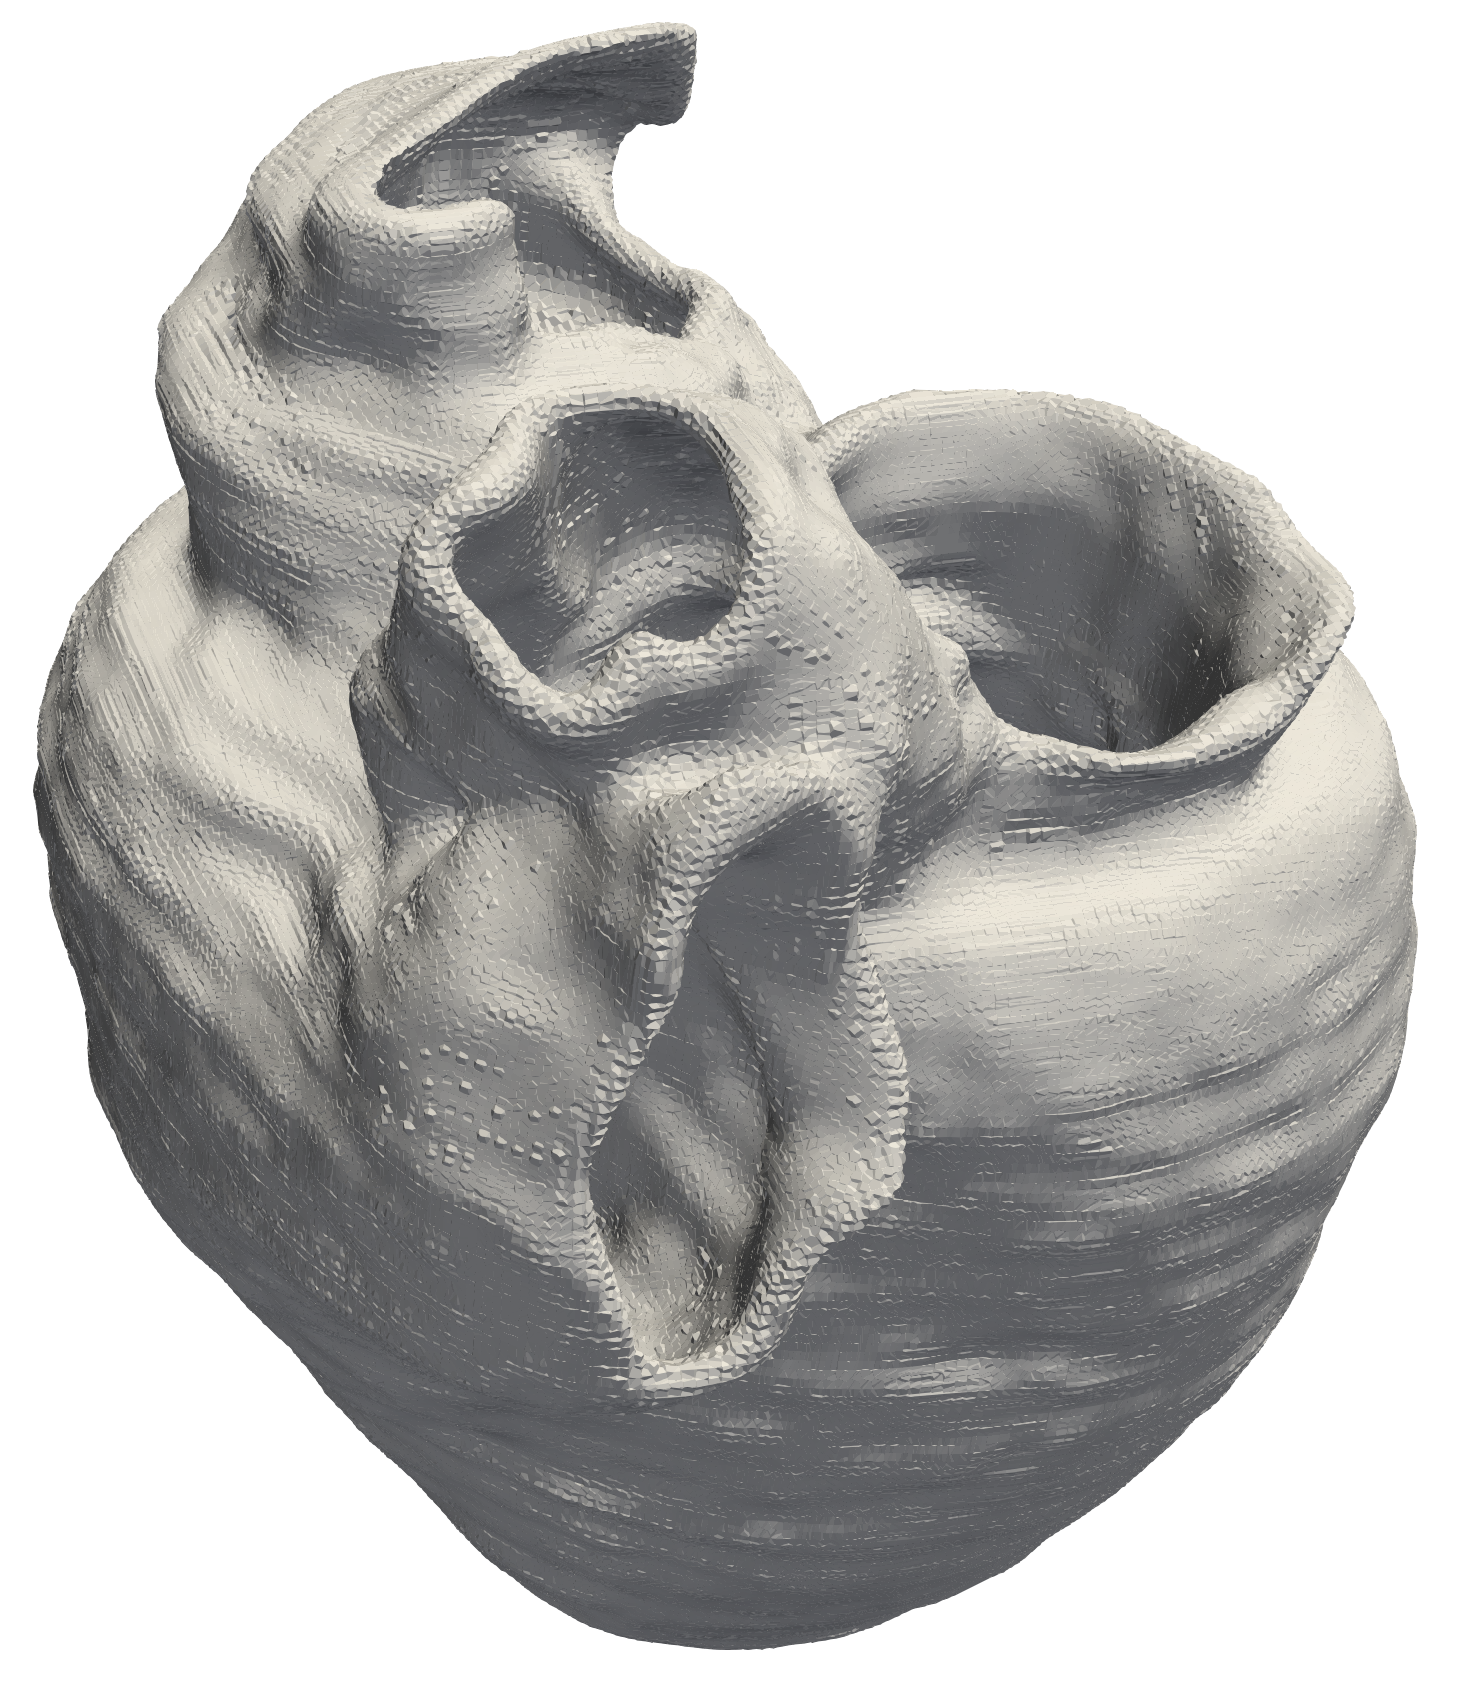
\includegraphics[scale=0.08]{media/2-shabaka/4-clean/1-init.png}
\label{fig:cross2-1}}		
\subfigure[]{%
		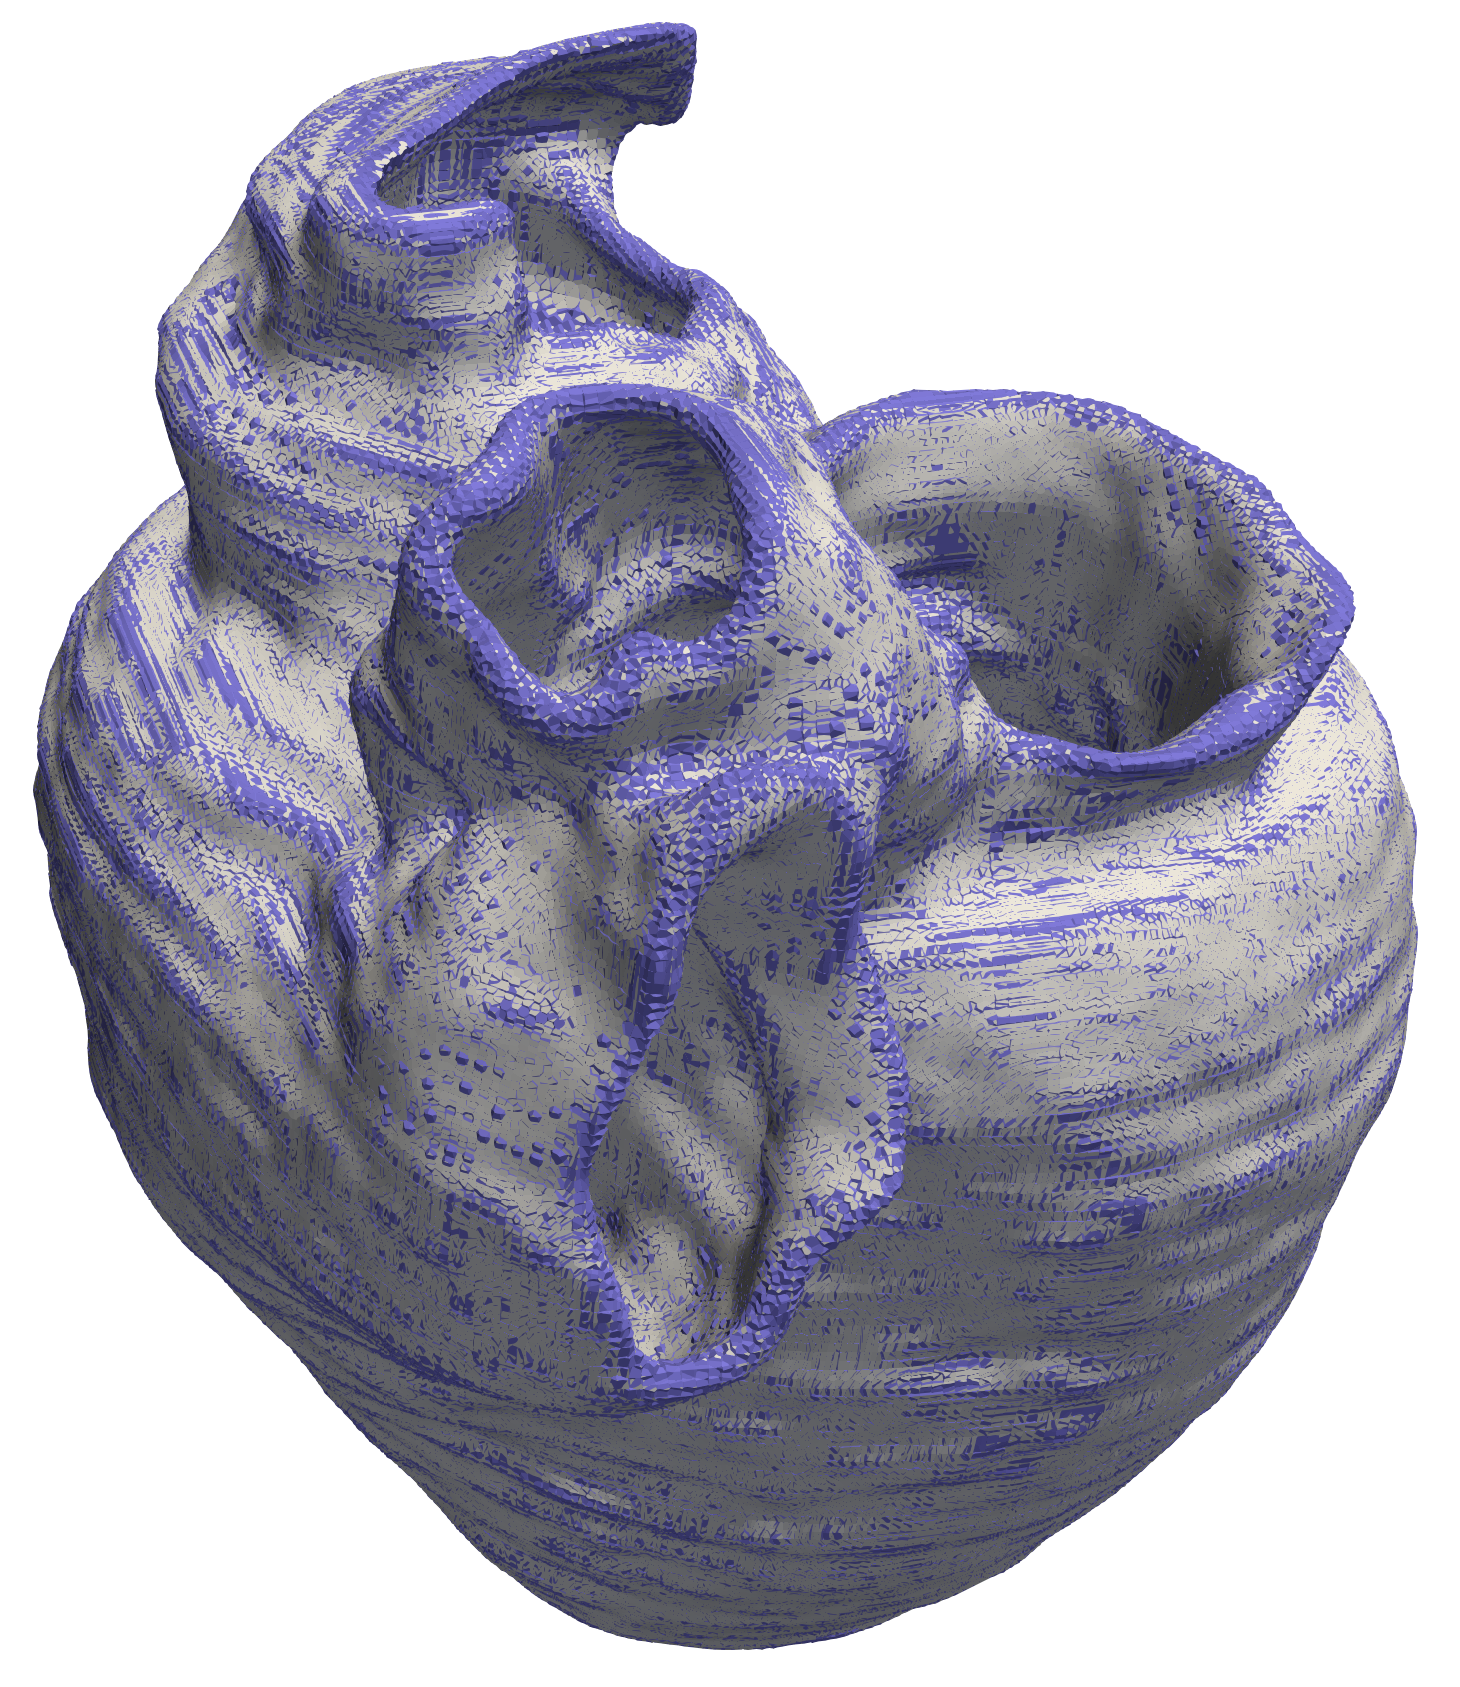
\includegraphics[scale=0.08]{media/2-shabaka/4-clean/2-badfacets.png}
\label{fig:cross2-2}}		
\subfigure[]{%
		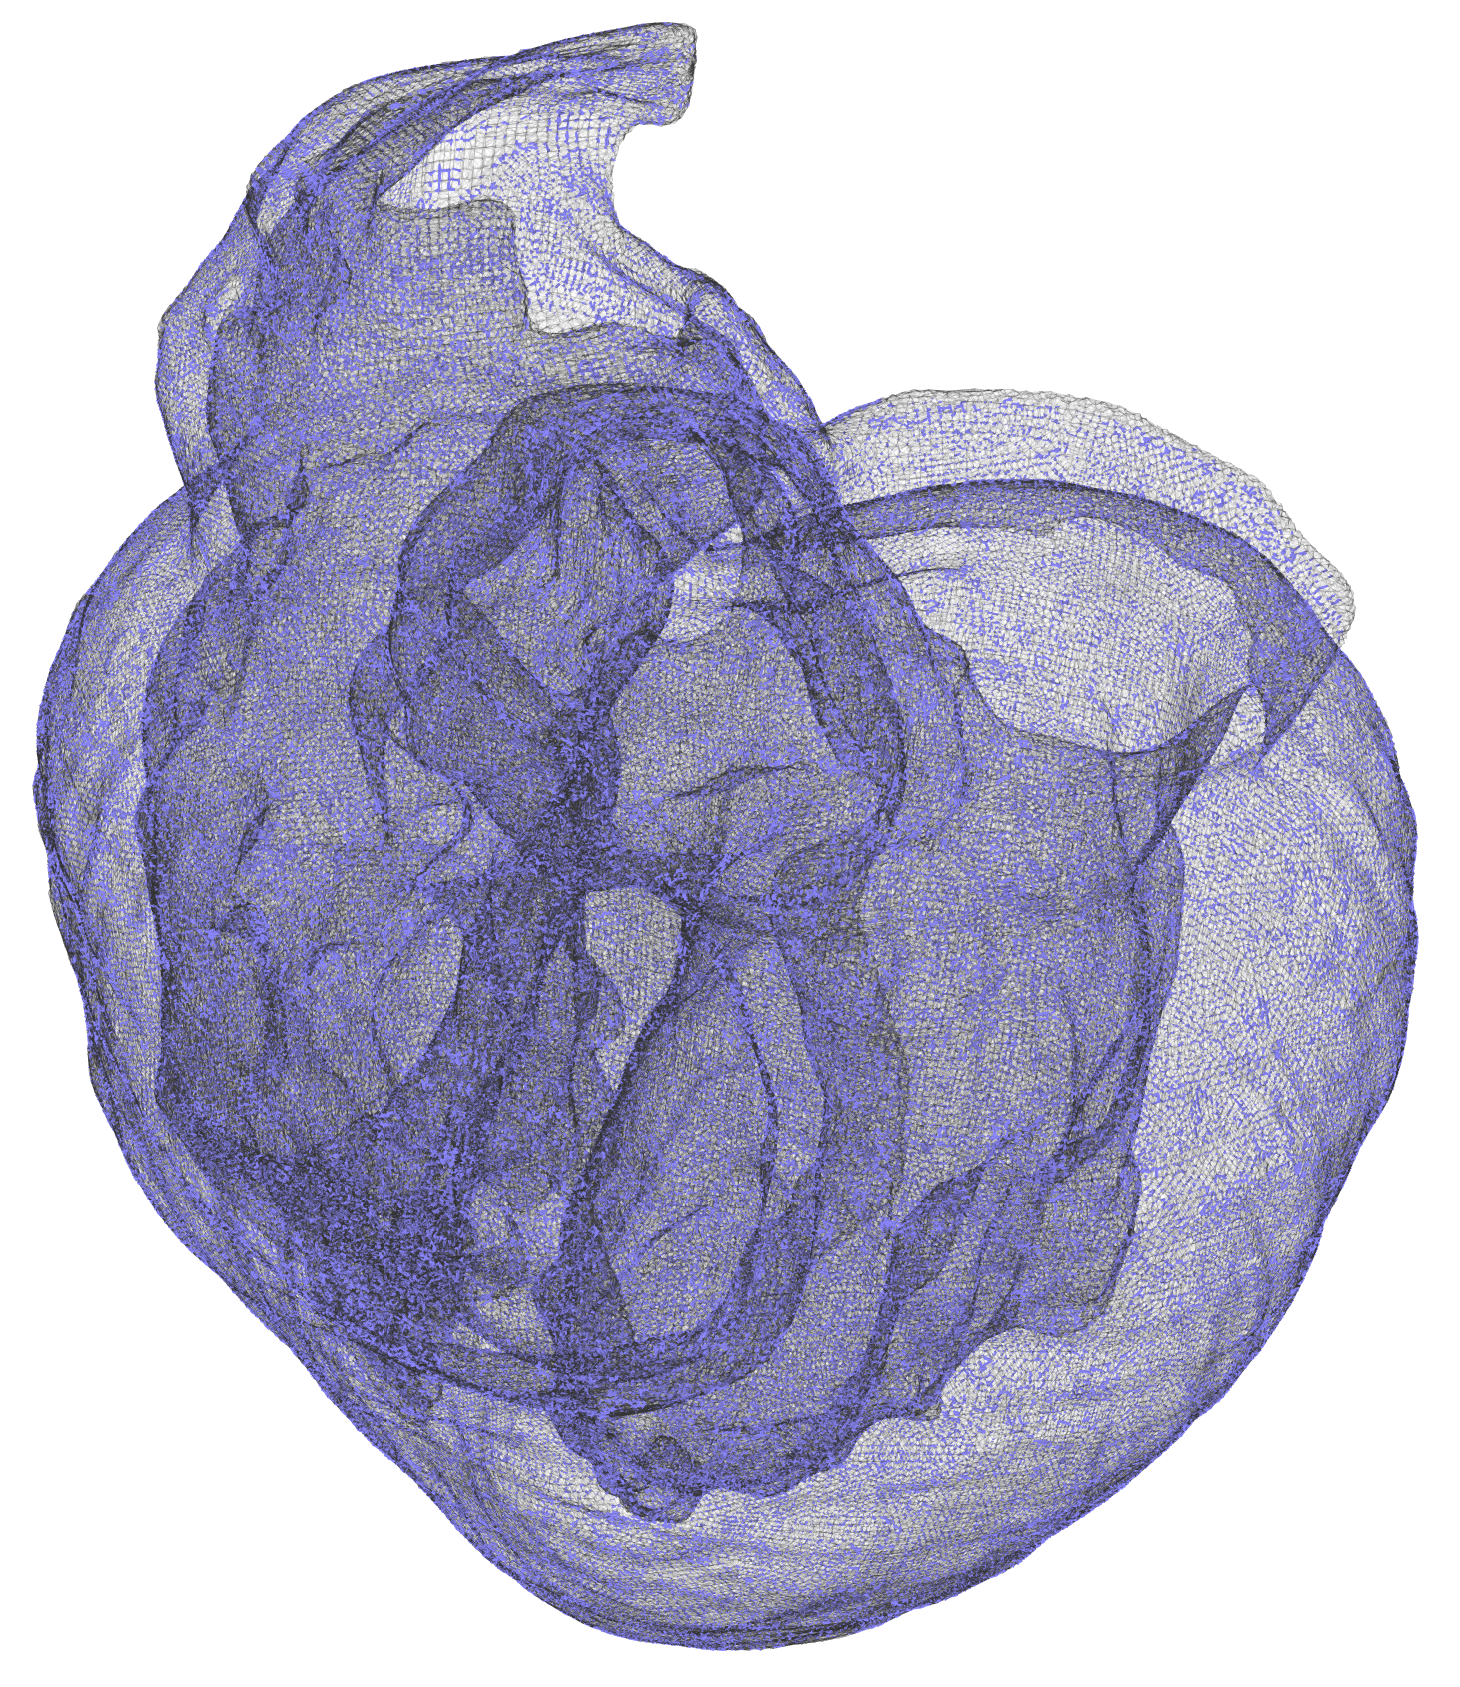
\includegraphics[scale=0.08]{media/2-shabaka/4-clean/3-badsegs.png}	
\label{fig:cross2-3}}						
\subfigure[]{%
		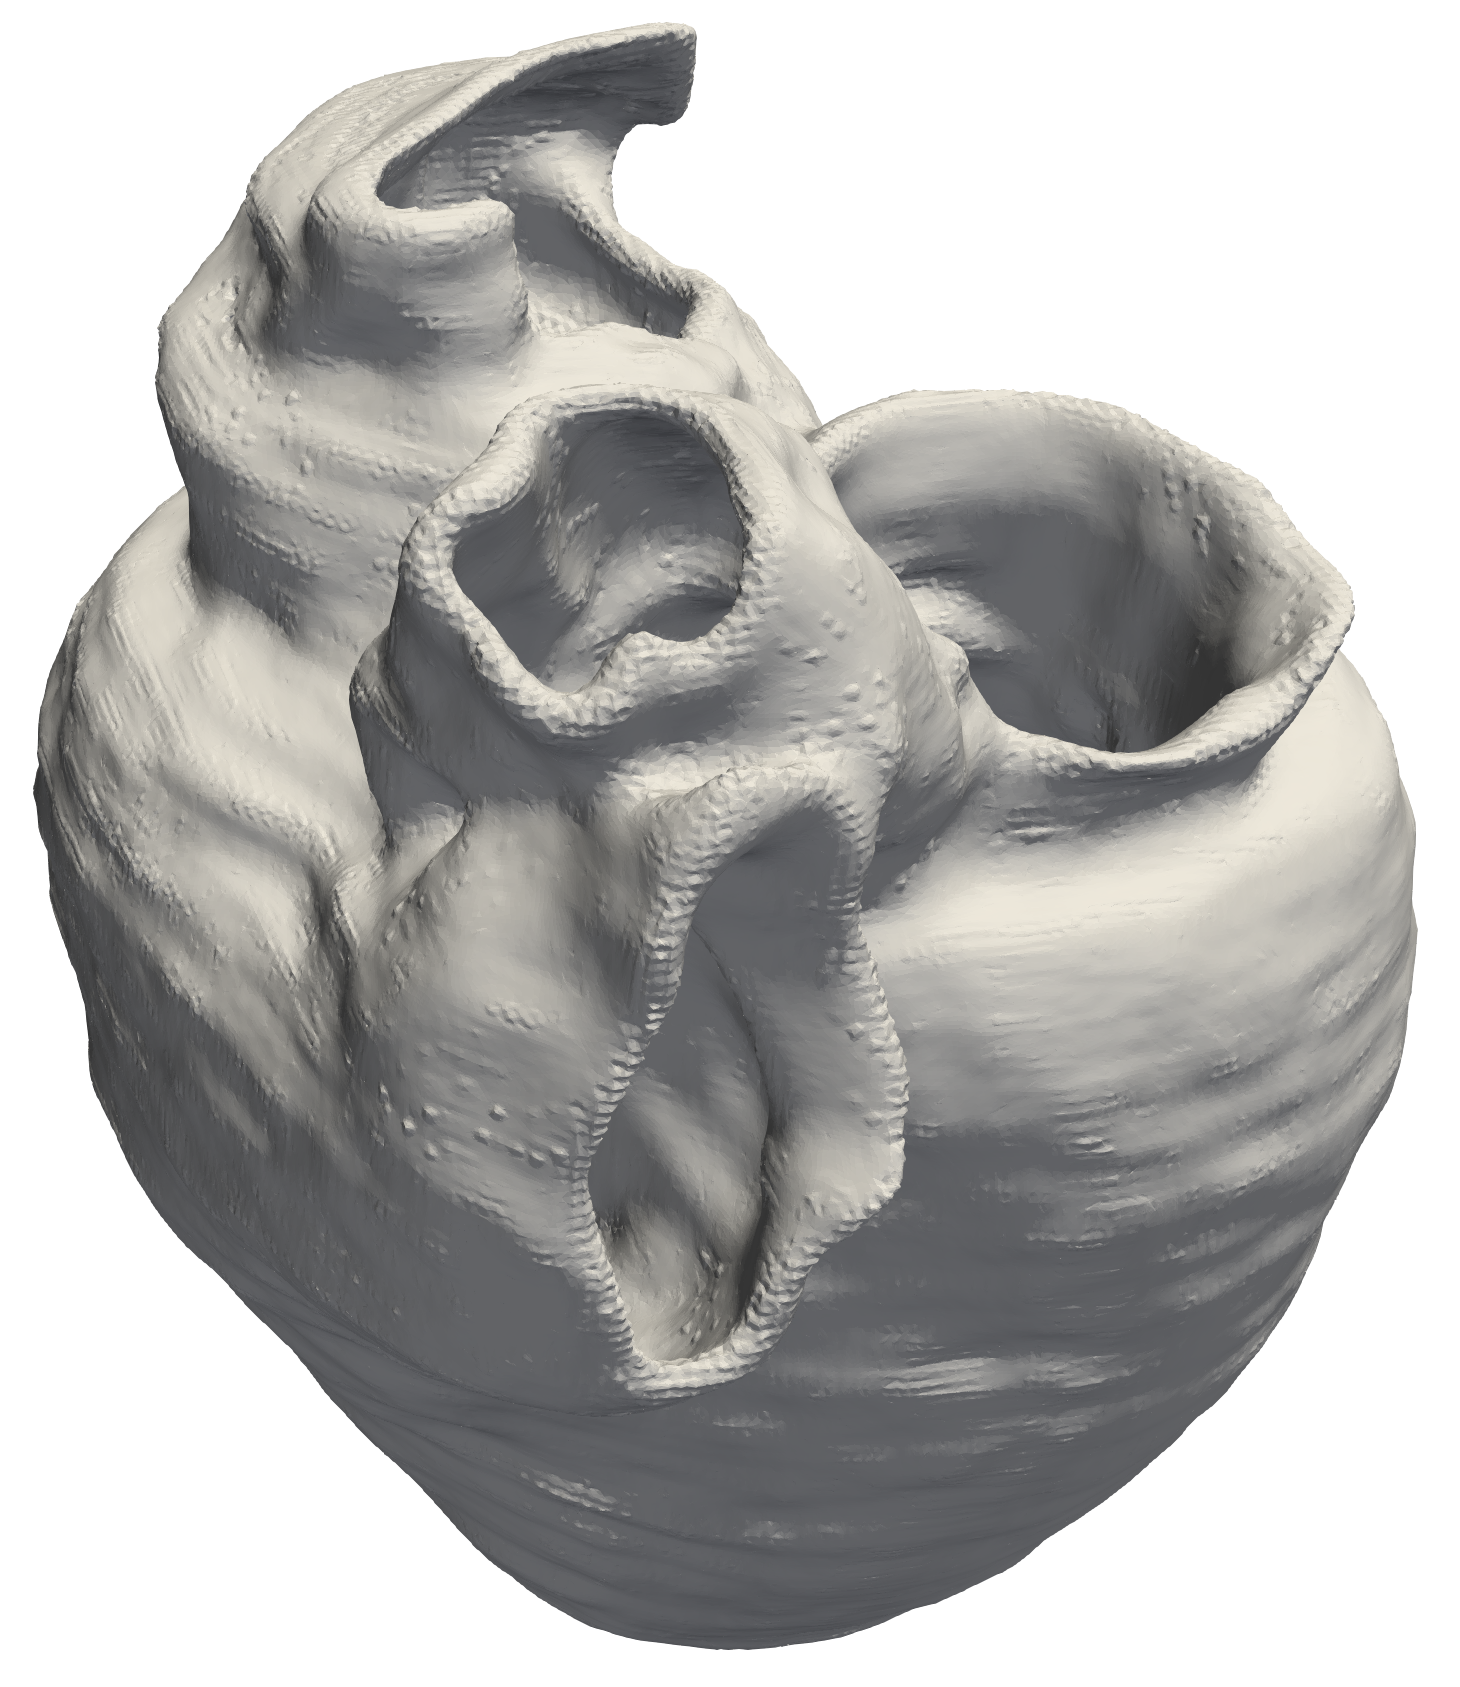
\includegraphics[scale=0.08]{media/2-shabaka/4-clean/4-fine.png}		
\label{fig:cross2-4}}		
%
\caption{Cleanup of undesirable ``cross-talk'' facets for surface of \textit{ex vivo} human heart (corresponding image mask generated from MRI data from Cardiovascular Research Grid~\cite{cvgg}): (a) initial surface following Voronoi-based surface reconstruction, (b) identification of ``cross-talk'' facets, (c) identification of edges to be collapsed, (d) final cleaned surface}
\label{fig:cross2}
\end{figure}
\noindent For the vast majority of ``bad-edge'' networks, the collapse technique results in a smoother surface that remains closed and manifold. For regions of high-curvature, there is a small set of cases in which the cleanup step may cause the surface to become non-manifold. The topology of particular networks of bad edges that cause this phenomenon are identified and are not collapsed to preserve the manifold property. The current approach thus is unable to alleviate the issue of ``cross-talk'' facets in regions of high curvature. Fortunately, these remaining artifacts are small enough that the ensuing decimation step removes them. \\ \\
%
Handling regions of curvature or even sharp corners and edges can certainly be done, though. The technique would involve including additional templates in the boundary approximation step that would allow more than two Voronoi sites to be generated for each sampling window. For example, three Voronoi sites can be used to produce an edge, and four sites can be used to produce a corner. This would significantly improve the point cloud approximation of the underlying surface, perhaps to a degree that the collapsing technique described would remove all cross-talk facets with no concern of losing manifoldness at all.

\subsubsection{Surface Decimation}

Surface \textit{decimation} is performed to reduce the surface mesh to a practical resolution without significantly changing the geometry. The philosophy in image-based meshing, surface extraction, and surface reconstruction is typically to make use of as much information as available to construct a mesh of the highest fidelity possible, and only then to address the practical consideration of mesh resolution for simulation purposes. The challenge then becomes decimating in a manner that does not lose more features from the original surface than is desired. For the purposes of this algorithm, decimation is performed using the code \textit{ACVD}~\cite{valette_2004, valette_2008}, which clusters vertices and triangles to generate a coarser surface mesh whose resulting triangles exhibit excellent aspect ratio. The approach does not preserve sharp edges or corners, however; feature-preserving decimation is still very much an active area of research.

\subsubsection{Results}

Results of the entire surface generation procedure described in this chapter are shown in~\figref{shabakaseq} for the \textit{ex vivo} human heart example. The optimal parameters identified for robust surface generation are shown in~\tabref{Mod5}. The algorithm was rigorously tested with these parameters to produce closed, manifold surfaces for a wide variety of examples, as is shown in in the following section.

\begin{table}[]
 \centering
   \begin{tabular}{|c||c|c|}
   \hline 
   \textbf{Variable} & \textbf{Description} & \textbf{Value} \\ \hline \hline
   $R_{\mathcal{W}}$ & window radius (in voxels) & 5 \\ \hline
   $d_{\mathcal{W}}$ & sampling distance between adjacent windows (in voxels) & 2 \\ \hline
   \multirow{2}{*}{$\overline{k}_{\mathcal{M}}$ \rule{0mm}{4mm}} & threshold for acceptable ratio of voxels in & \multirow{2}{*}{0.925} \\
   {} & window $\mathcal{W}$ belonging to material $m$ & {} \\ \hline
   $\beta_0$ & weighting coefficient for zeroth moment of volume & 0.5 \\ \hline
   $\beta_1$ & weighting coefficient for first moment of volume & 0.3 \\ \hline   
   $\varepsilon$ & tolerance for minimization of function $\mathcal{F}$ & $10^{-14}$ \rule{0mm}{4mm} \\ \hline
   $\overline{\mathcal{F}}$ \rule{0mm}{4mm} & largest acceptable value of function $\mathcal{F}$ & $0.15$ \\ \hline
   \multirow{2}{*}{$b$} & distance between boundary normal and & \multirow{2}{*}{$1.1$} \\
   {} & corresponding Voronoi site pair (in voxels) & {} \\ \hline
\end{tabular}
\caption{Optimal parameter values for b-rep generation}
\label{tab:Mod5}
\end{table}

\begin{figure}[]
\centering
\subfigure[]{%
		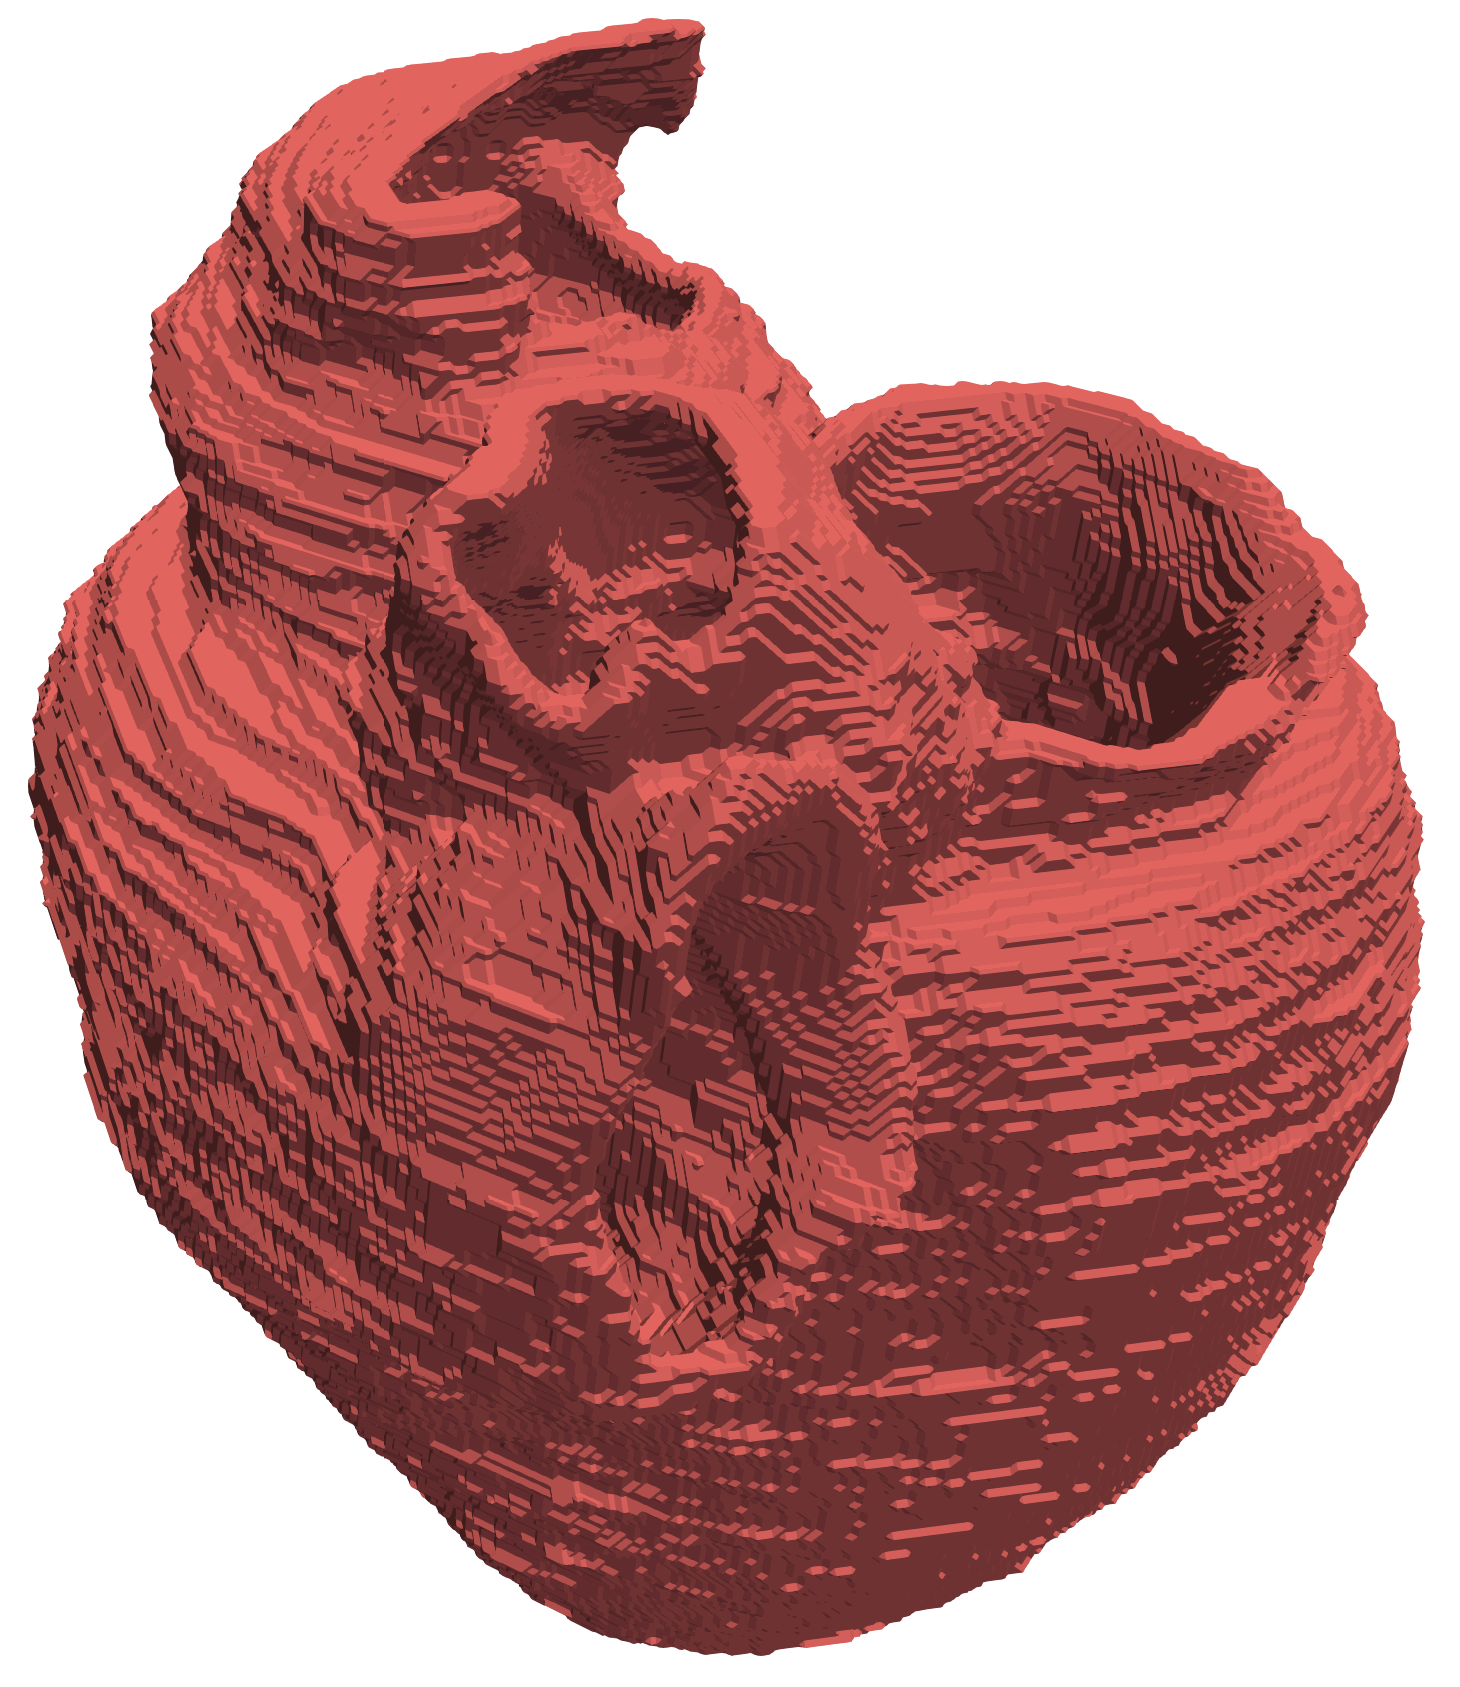
\includegraphics[scale=0.08]{media/2-shabaka/2-surf/1-seg.png}
\label{fig:shabakaseq1}}
\subfigure[]{%
		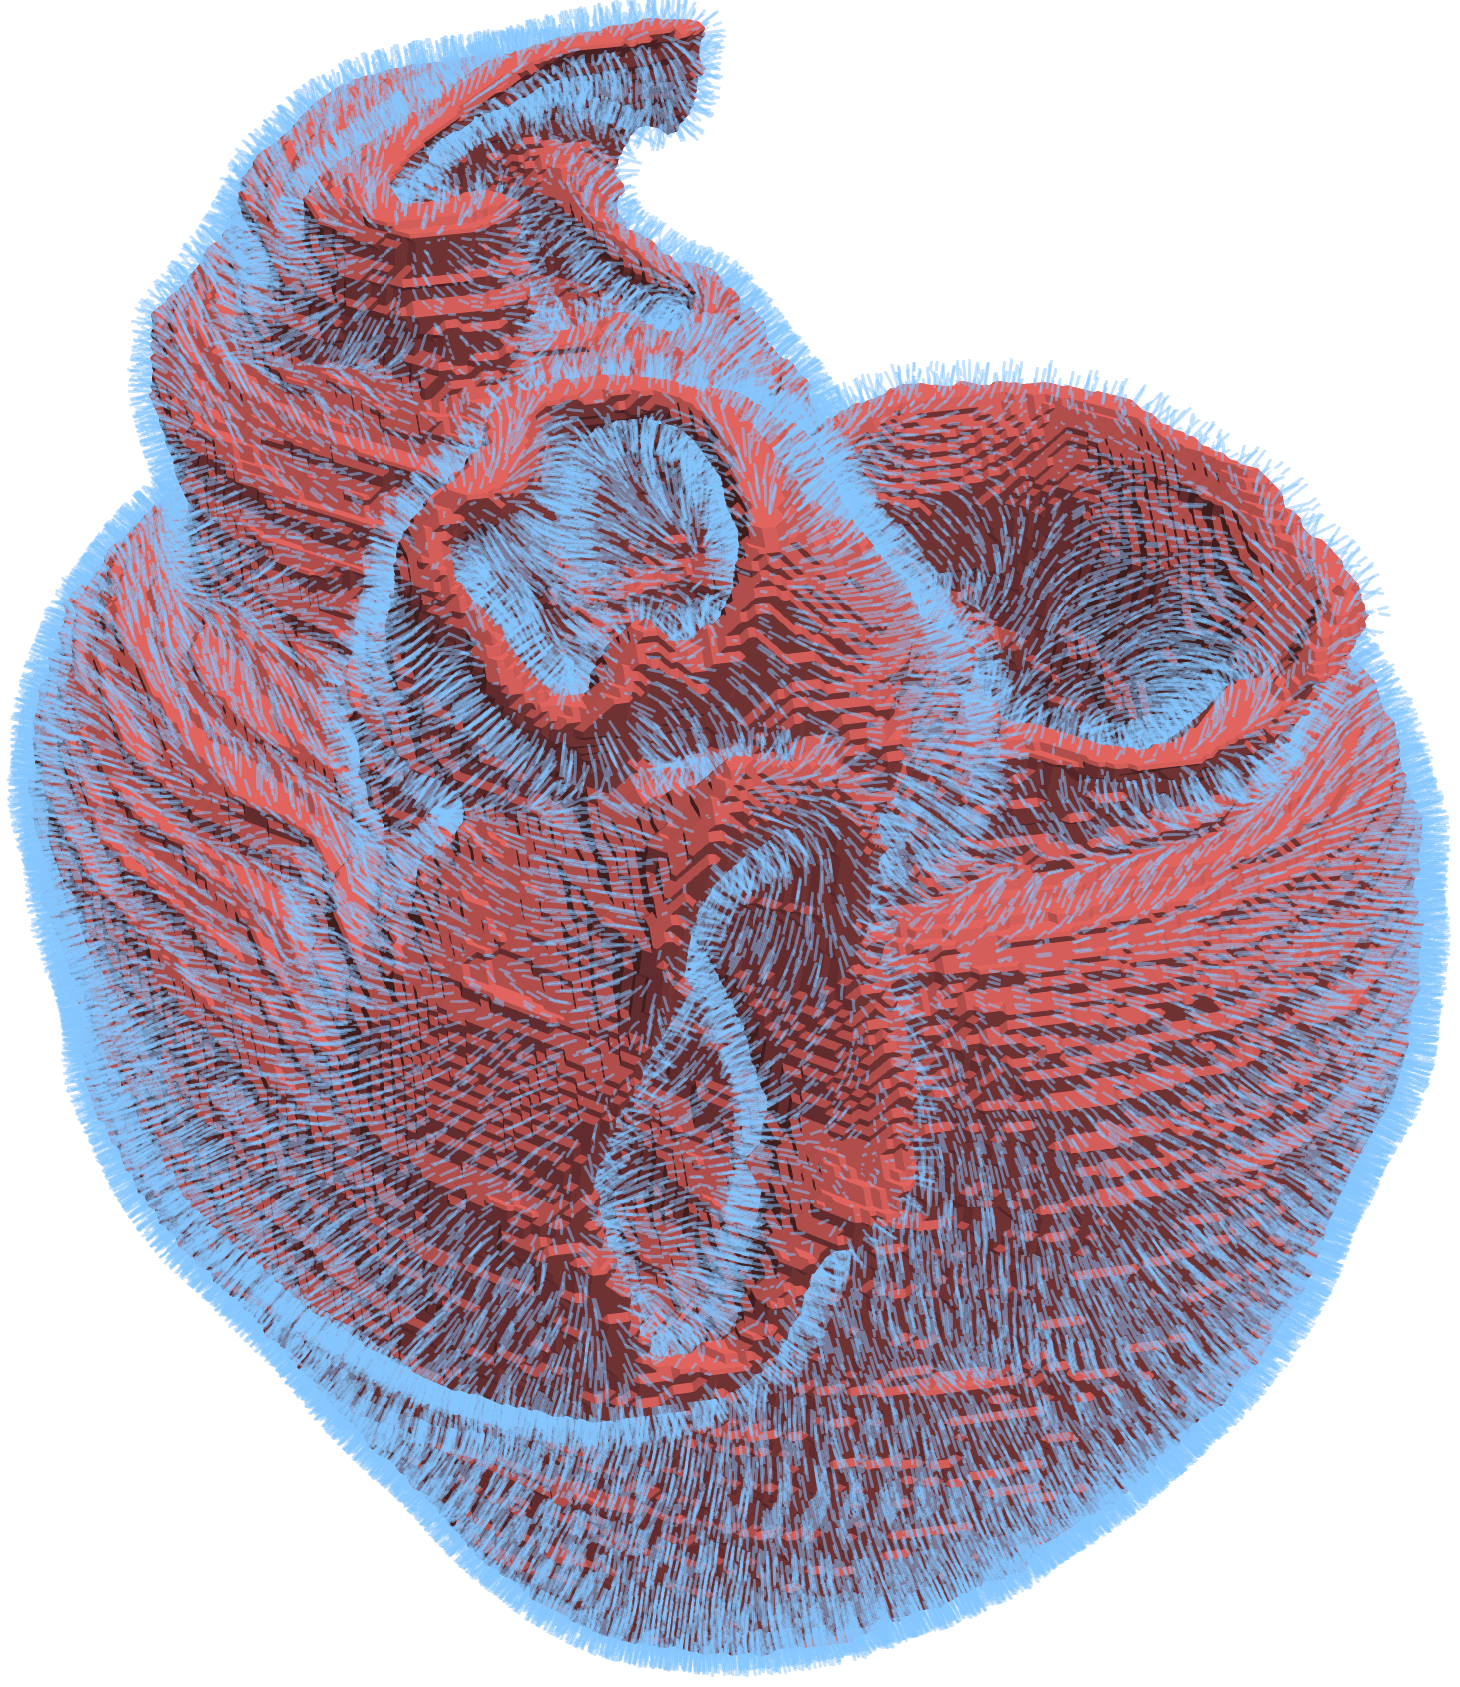
\includegraphics[scale=0.08]{media/2-shabaka/2-surf/2-normals.png}
\label{fig:shabakaseq2}}
\subfigure[]{%
		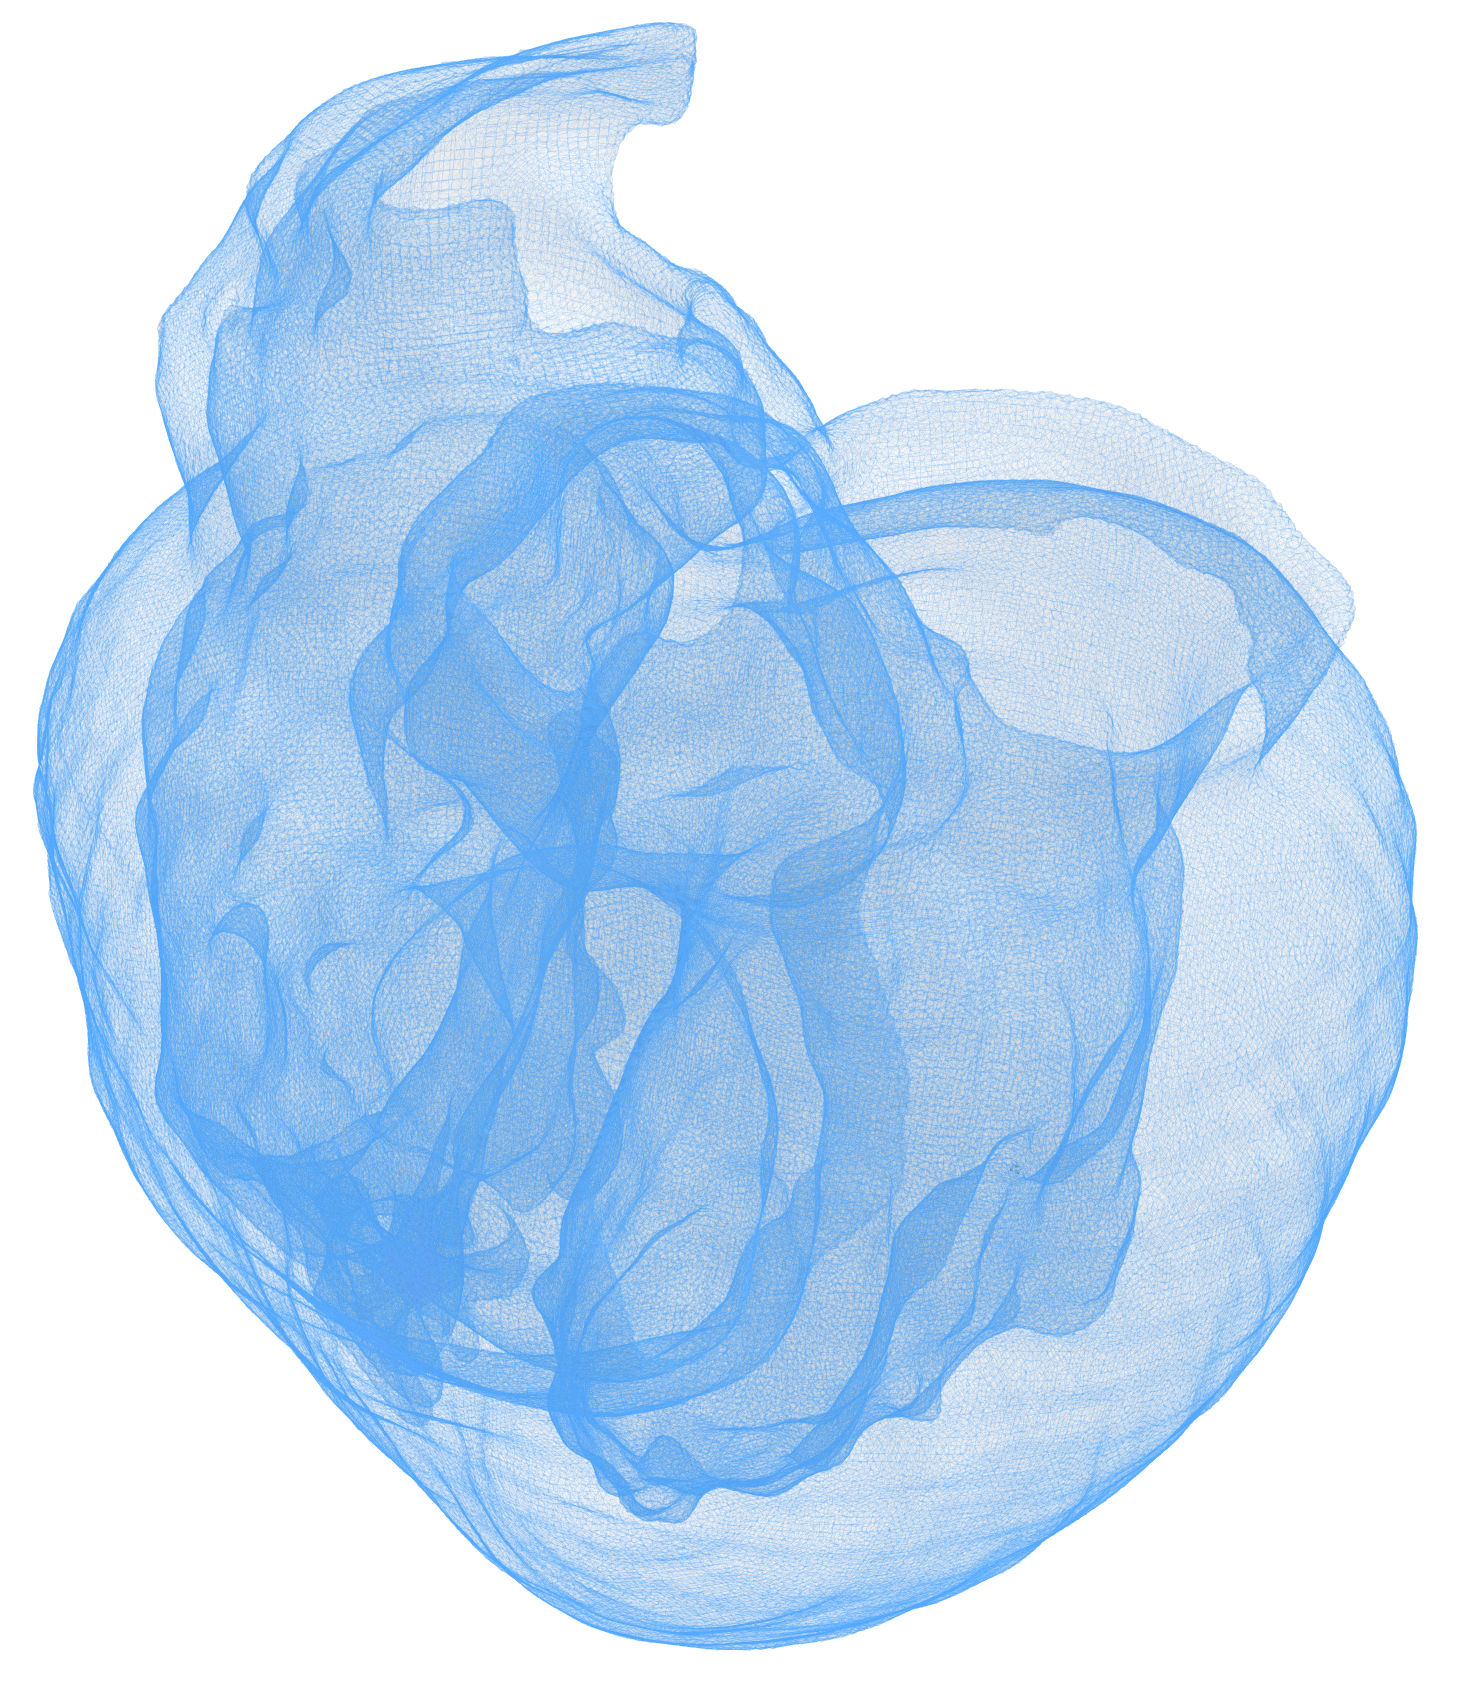
\includegraphics[scale=0.08]{media/2-shabaka/2-surf/3-ptcloud.png}
\label{fig:shabakaseq3}}
\\
\subfigure[]{%
		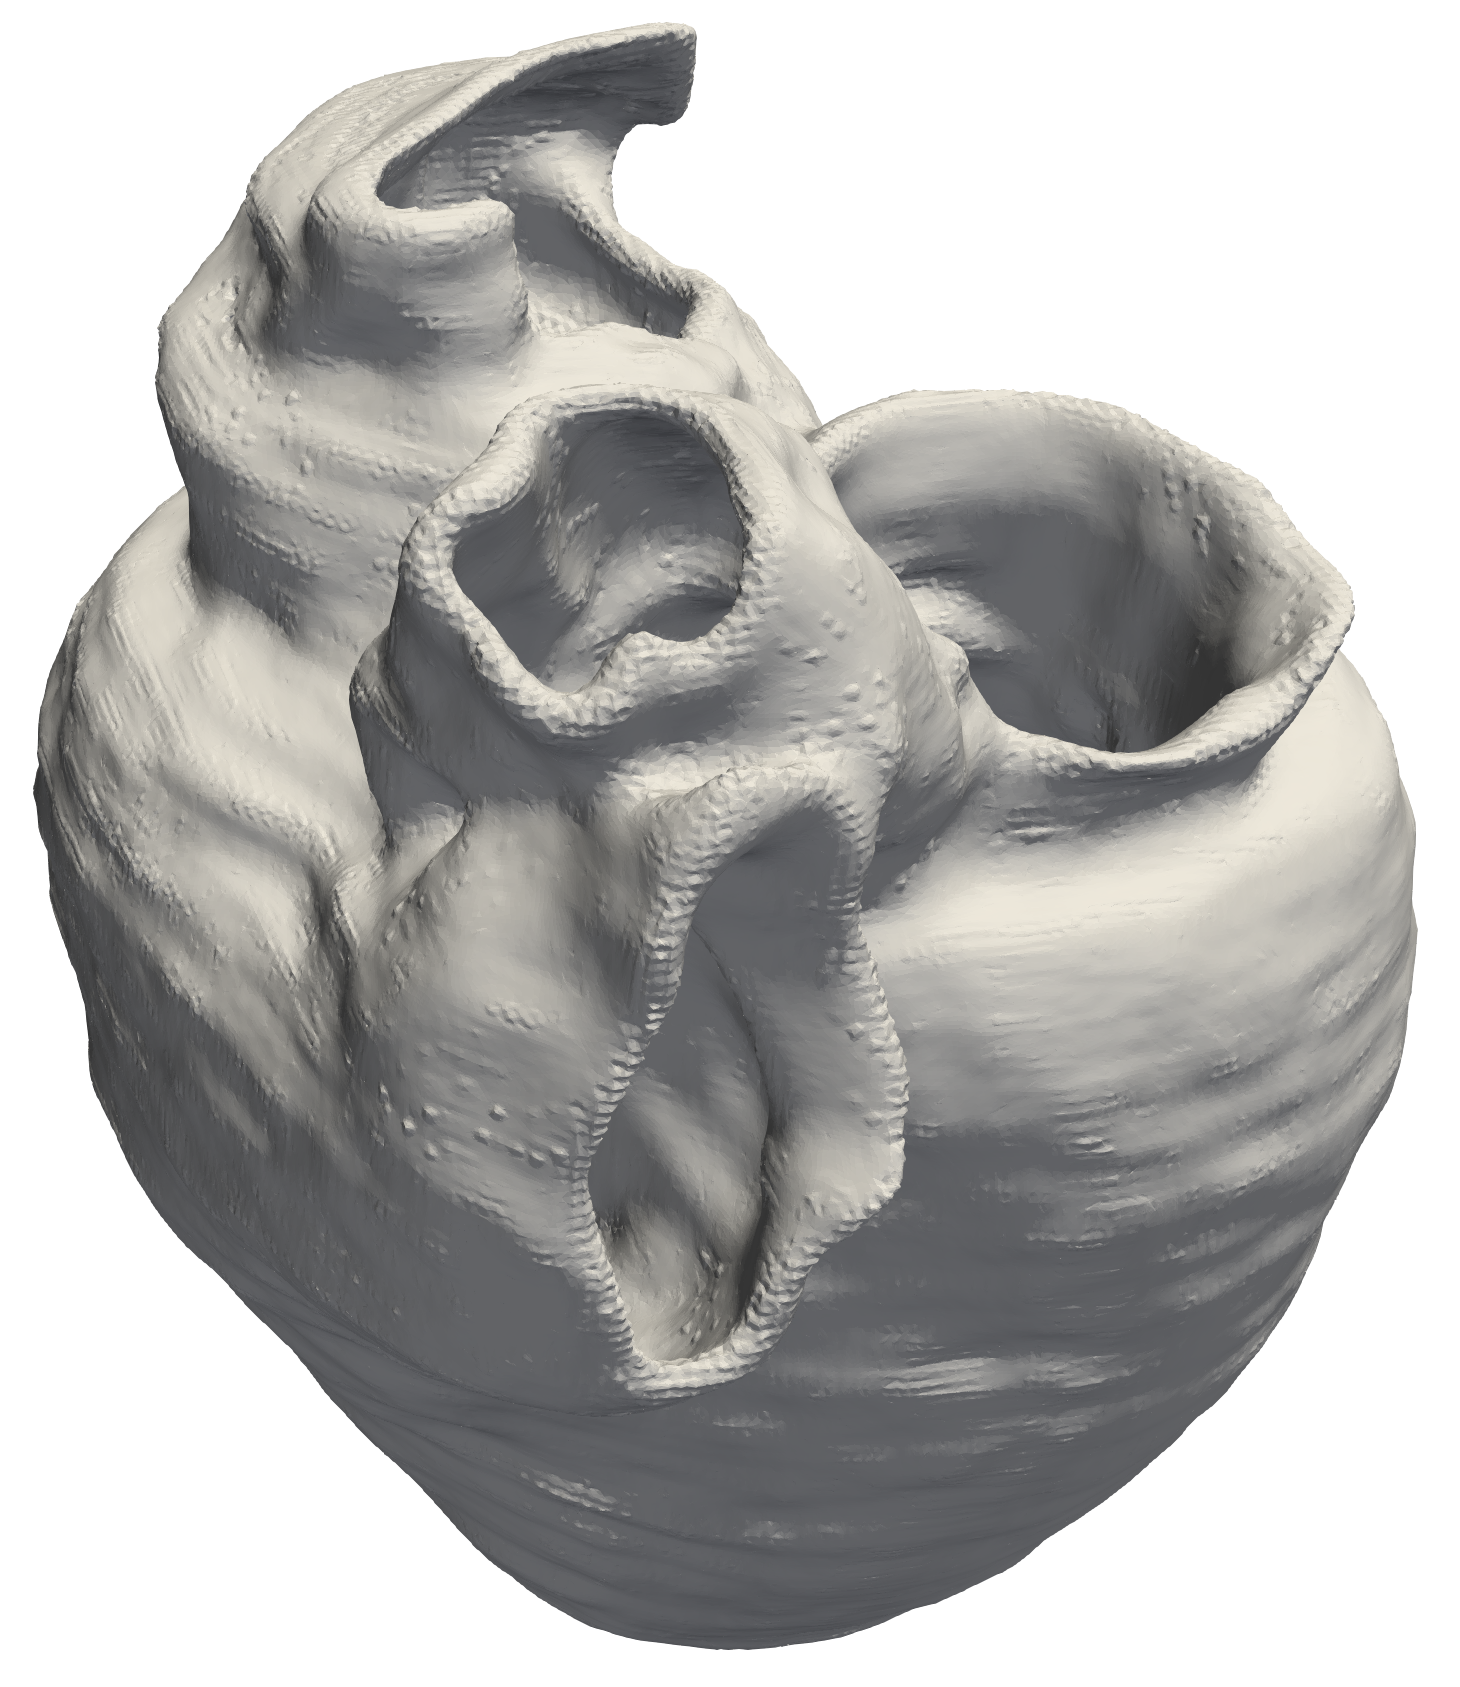
\includegraphics[scale=0.08]{media/2-shabaka/2-surf/4-finesurf.png}
\label{fig:shabakaseq4}}
\subfigure[]{%
		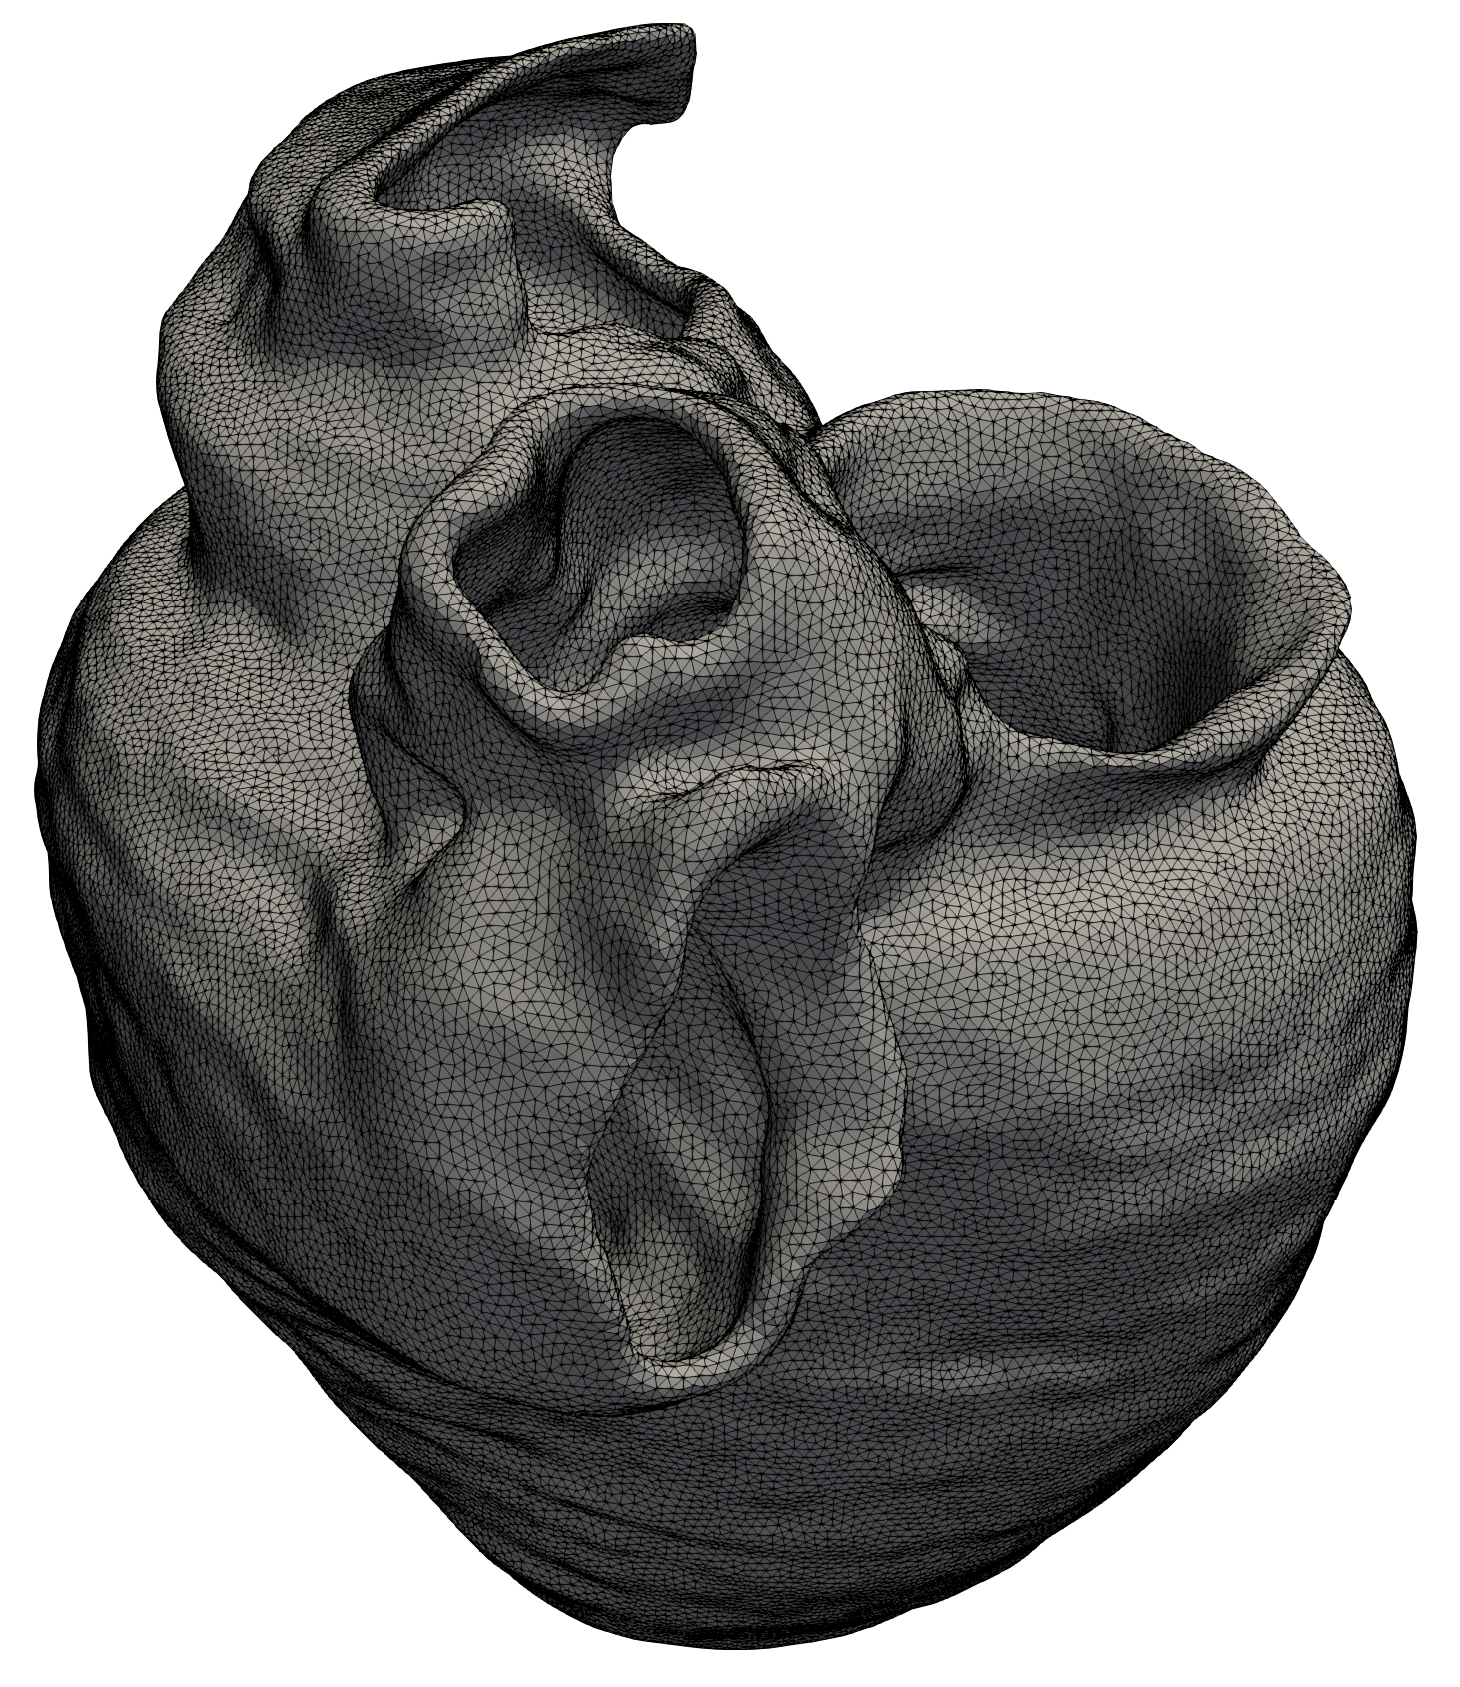
\includegraphics[scale=0.08]{media/2-shabaka/2-surf/5-surf.png}
\label{fig:shabakaseq5}}
%
\caption{(a) Segmented image, (b) point/normal placement, (c) oriented point cloud (normals not shown), c) cleaned surface mesh generated from Voronoi partition (edges not shown), and d) final decimated surface}
\label{fig:shabakaseq}
\end{figure}

%%%%%%%%%%%%%%%%%%%%%%%%%%%%%%%%%%%%%%%%%%%%%%%
%%%%%%%%%%%%%%%%%%%%%%%%%%%%%%%%%%%%%%%%%%%%%%%

